\documentclass[10pt,journal,compsoc]{IEEEtran}

\ifCLASSOPTIONcompsoc
  \usepackage[nocompress]{cite}
\else
  \usepackage{cite}
\fi
\usepackage{amsmath,amssymb}
\usepackage{graphicx}
\usepackage{array}
\usepackage{booktabs}
\usepackage{url}
\usepackage{microtype}
\usepackage[hidelinks]{hyperref}
\usepackage{xcolor}
\usepackage{fvextra}
\fvset{breaklines=true,breakanywhere=true,breakautoindent=false,breakindent=0pt,fontsize=\small}
\newcommand{\VerbBar}{|}
\newcommand{\VERB}{\Verb[commandchars=\\\{\}]}
\DefineVerbatimEnvironment{Highlighting}{Verbatim}{commandchars=\\\{\},breaklines=true,breakanywhere=true,breakautoindent=false,breakindent=0pt,fontsize=\small}
\newenvironment{Shaded}{}{}
\newcommand{\AlertTok}[1]{\textcolor[rgb]{1.00,0.00,0.00}{\textbf{#1}}}
\newcommand{\AnnotationTok}[1]{\textcolor[rgb]{0.38,0.63,0.69}{\textbf{\textit{#1}}}}
\newcommand{\AttributeTok}[1]{\textcolor[rgb]{0.49,0.56,0.16}{#1}}
\newcommand{\BaseNTok}[1]{\textcolor[rgb]{0.25,0.63,0.44}{#1}}
\newcommand{\BuiltInTok}[1]{\textcolor[rgb]{0.00,0.50,0.00}{\textbf{#1}}}
\newcommand{\CharTok}[1]{\textcolor[rgb]{0.25,0.44,0.63}{#1}}
\newcommand{\CommentTok}[1]{\textcolor[rgb]{0.38,0.63,0.69}{\textit{#1}}}
\newcommand{\CommentVarTok}[1]{\textcolor[rgb]{0.38,0.63,0.69}{\textbf{\textit{#1}}}}
\newcommand{\ConstantTok}[1]{\textcolor[rgb]{0.53,0.00,0.00}{#1}}
\newcommand{\ControlFlowTok}[1]{\textcolor[rgb]{0.00,0.44,0.13}{\textbf{#1}}}
\newcommand{\DataTypeTok}[1]{\textcolor[rgb]{0.56,0.13,0.00}{#1}}
\newcommand{\DecValTok}[1]{\textcolor[rgb]{0.25,0.63,0.44}{#1}}
\newcommand{\DocumentationTok}[1]{\textcolor[rgb]{0.73,0.13,0.13}{\textit{#1}}}
\newcommand{\ErrorTok}[1]{\textcolor[rgb]{1.00,0.00,0.00}{\textbf{#1}}}
\newcommand{\ExtensionTok}[1]{#1}
\newcommand{\FloatTok}[1]{\textcolor[rgb]{0.25,0.63,0.44}{#1}}
\newcommand{\FunctionTok}[1]{\textcolor[rgb]{0.02,0.16,0.49}{#1}}
\newcommand{\ImportTok}[1]{\textcolor[rgb]{0.00,0.50,0.00}{\textbf{#1}}}
\newcommand{\InformationTok}[1]{\textcolor[rgb]{0.38,0.63,0.69}{\textbf{\textit{#1}}}}
\newcommand{\KeywordTok}[1]{\textcolor[rgb]{0.00,0.44,0.13}{\textbf{#1}}}
\newcommand{\NormalTok}[1]{#1}
\newcommand{\OperatorTok}[1]{\textcolor[rgb]{0.40,0.40,0.40}{#1}}
\newcommand{\OtherTok}[1]{\textcolor[rgb]{0.00,0.44,0.13}{#1}}
\newcommand{\PreprocessorTok}[1]{\textcolor[rgb]{0.74,0.48,0.00}{#1}}
\newcommand{\RegionMarkerTok}[1]{#1}
\newcommand{\SpecialCharTok}[1]{\textcolor[rgb]{0.25,0.44,0.63}{#1}}
\newcommand{\SpecialStringTok}[1]{\textcolor[rgb]{0.73,0.40,0.53}{#1}}
\newcommand{\StringTok}[1]{\textcolor[rgb]{0.25,0.44,0.63}{#1}}
\newcommand{\VariableTok}[1]{\textcolor[rgb]{0.10,0.09,0.49}{#1}}
\newcommand{\VerbatimStringTok}[1]{\textcolor[rgb]{0.25,0.44,0.63}{#1}}
\newcommand{\WarningTok}[1]{\textcolor[rgb]{0.38,0.63,0.69}{\textbf{\textit{#1}}}}
\newcommand{\pandocbounded}[1]{#1}
\usepackage{calc}
\newcommand{\real}[1]{#1}
\providecommand{\tightlist}{%
  \setlength{\itemsep}{0pt}\setlength{\parskip}{0pt}}
\usepackage{tikz}
\usetikzlibrary{arrows.meta,positioning}


\title{SkyBridge Compass: A Crypto-Agile Peer-to-Peer Remote Desktop and File Transfer System with Post-Quantum Readiness on Apple Platforms}
\author{Zi'ang Li\thanks{Independent Researcher. E-mail: 2403871950@qq.com}}

\begin{document}

\IEEEtitleabstractindextext{%
\begin{abstract}
Peer-to-peer remote desktop and file transfer
systems increasingly operate across heterogeneous devices, untrusted
networks, and long lifecycles in which cryptographic assumptions may
expire faster than products. Yet ``post-quantum readiness'' is often
treated as a one-off algorithm swap rather than a migration problem with
downgrade resistance, auditability, and reproducibility requirements.
This paper presents SkyBridge Compass, a crypto-agile P2P system that
explicitly separates (i) negotiated cryptographic suites, (ii)
platform-specific provider backends, and (iii) a policy layer that
governs when (and whether) classic fallback is permissible. We introduce
an actor-isolated handshake state machine with deterministic failure
semantics and structured security-event emission, enabling end-to-end
audit trails for downgrade, identity mismatch, and signature
verification failures. We evaluate three configurations on macOS 26.x:
classic (X25519 + Ed25519), PQC via liboqs (ML-KEM-768 + ML-DSA-65), and
PQC via native CryptoKit (ML-KEM-768 + ML-DSA-65). End-to-end handshake
completion latency (including event emission overhead) is 1.81 ms (p95
2.09 ms) for classic, 6.32 ms (p95 8.15 ms) for liboqs PQC, and 11.02 ms
(p95 16.15 ms) for CryptoKit PQC over N=1000 iterations. The wire-format
size grows from 819 B (classic) to 12,155 B (PQC), and we provide a
conservative projection for a hybrid X-Wing-style exchange of
approximately 12.4 KB. Beyond performance, we validate security-centric
properties under fault injection and downgrade workloads, and we provide
scripts and tests that reproduce all primary figures and tables from
released artifacts.
\end{abstract}

\begin{IEEEkeywords}
post-quantum cryptography, crypto agility, downgrade resistance, secure handshake, peer-to-peer systems, remote desktop, Apple platforms, auditability, reproducibility.
\end{IEEEkeywords}}

\maketitle
\IEEEdisplaynontitleabstractindextext

\IEEEraisesectionheading{\section{Introduction}\label{sec:introduction}}

Peer-to-peer (P2P) remote desktop and file transfer systems must
establish secure sessions under adversarial network conditions, device
churn, and multi-year lifecycles. These systems face a practical
tension: users demand ``it just works'' pairing across heterogeneous
stacks, while defenders require that cryptographic negotiation remains
robust against downgrade and implementation-level failure modes.
Post-quantum cryptography (PQC) increases this tension. Larger messages,
higher computational cost, and uneven platform support make fallback
tempting---yet fallback is exactly where silent downgrade and
unverifiable behavior tend to hide.

Existing secure-channel designs and frameworks provide mature
cryptographic building blocks, but they do not, by default, solve the
migration problem an implementer actually faces: (i) selecting among
classic/PQC/hybrid suites across platform strata, (ii) guaranteeing that
policy (e.g., ``require PQC'') is enforced at the entry points where
callers cannot accidentally violate it, (iii) ensuring deterministic
failure semantics under timeouts, reorder/duplication, and malformed
inputs, and (iv) emitting security-relevant telemetry that can be
audited without turning the system into a logging minefield. In
practice, many systems either hard-code a single suite, or allow
``compatibility'' to creep into negotiation in ways that are hard to
reason about and harder to verify.

This paper addresses these gaps with SkyBridge Compass, a crypto-agile
P2P system designed for explicit PQC migration and auditability on Apple
platforms. The core idea is to treat crypto agility as a layered
contract: negotiated suites define the protocol surface; provider
backends implement suites using platform-native or portable
cryptography; and a policy layer governs fallback and produces
structured evidence when (and only when) downgrade occurs. We complement
this design with an actor-isolated handshake driver that enforces
one-shot completion, timeouts, and sensitive-material zeroization,
yielding deterministic outcomes even under adverse transport behaviors.

\subsection{Contributions}\label{a.-contributions}

Contributions (reviewer-facing, evidence-backed):

\begin{enumerate}
\def\labelenumi{\arabic{enumi}.}
\item
  We turn PQC migration from a narrative into an enforceable contract by
  making downgrade and legacy-compatibility decisions explicit,
  testable, and auditable rather than implicit ``best-effort'' fallback.
  (Fig.~\ref{fig:downgrade-matrix}; Table~\ref{tab:security-contract};
  PolicyDowngradeBenchTests,
  LegacyFallbackPreconditionTests)
\item
  We design a crypto-agile P2P handshake that cleanly separates suite
  negotiation, transcript binding, and protocol-signature keys,
  preventing ``suite says PQC but keys stay classical'' class of
  integration bugs. (Fig.~\ref{fig:handshake-sequence};
  Table~\ref{tab:security-contract};
  ProtocolSignatureRegressionTests, TranscriptIntegrityPropertyTests)
\item
  We provide migration safety with measurable coverage by enumerating
  legacy/PQC strata and validating acceptance/rejection boundaries under
  fault injection instead of relying on informal compatibility claims.
  (Table~\ref{tab:legacy-precondition};
  Table~\ref{tab:failure-mode}; HandshakeFaultInjectionBenchTests)
\item
  We harden correctness under concurrency by an actor-isolated state
  machine with idempotent transitions and bounded retries, eliminating
  double-resume and state desynchronization failure modes.
  (Fig.~\ref{fig:handshake-state-machine};
  Table~\ref{tab:security-contract}; HandshakeDriverTests)
\item
  We make evaluation reproducible by shipping a benchmark harness that
  reports distributional statistics (p50/p95/p99) over large-N runs and
  links each metric back to a concrete failure taxonomy.
  (Fig.~\ref{fig:policy-fallback};
  Tables~\ref{tab:handshake-latency}--\ref{tab:handshake-sizes};
  HandshakeBenchmarkTests, MessageSizeSnapshotTests)
\end{enumerate}

\subsection{Paper Organization}\label{b.-paper-organization}

Section II reviews related work on P2P pairing, negotiation, and PQC
migration. Section III details system architecture and protocol design.
Section IV presents the handshake state machine. Section V presents the
security model and guarantees. Section VI describes implementation
details and platform instantiation. Section VII outlines evaluation
methodology and metrics. Section VIII discusses limitations and future
work, and Section IX concludes.



\section{Related Work}

\subsection{Peer-to-Peer Device
Pairing}\label{a.-peer-to-peer-device-pairing}

Device pairing protocols have evolved from simple PIN-based schemes to
sophisticated cryptographic handshakes. Bluetooth Secure Simple Pairing
(SSP) \cite{ref2} introduced numeric comparison and passkey entry modes, but
remains vulnerable to man-in-the-middle attacks during the initial
exchange. Apple's Continuity protocols leverage iCloud identity for
cross-device authentication \cite{ref3}, but require cloud connectivity and
Apple ID enrollment.

PAKE (Password-Authenticated Key Exchange) protocols, particularly
SPAKE2+ \cite{ref4}, enable secure pairing using low-entropy secrets without
exposing them to offline dictionary attacks. PAKE-based pairing is
considered as an alternative to our current PIN-comparison approach for
the initial pairing ceremony; however, the pairing phase is out of scope
of this paper's session handshake protocol. Our system uses visual PIN
comparison during initial pairing while supporting hardware-backed key
storage through Secure Enclave for subsequent sessions.

\subsection{Cryptographic Agility and
Negotiation}\label{b.-cryptographic-agility-and-negotiation}

The concept of cryptographic agility---designing systems to accommodate
algorithm changes without architectural overhaul---has gained prominence
as cryptographic standards evolve \cite{ref5}. TLS 1.3 and QUIC exemplify
suite negotiation and downgrade defenses by binding the selected
parameters into signed transcripts or transport parameters \cite{ref6},
\cite{ref18}. However, agility introduces complexity: systems must handle
negotiation failures, prevent downgrade attacks, and maintain backward
compatibility across heterogeneous peers.

Barker and Roginsky \cite{ref7} provide NIST guidelines for transitioning to
post-quantum algorithms, emphasizing hybrid approaches that combine
classical and quantum-resistant primitives. Our CryptoProvider
architecture directly implements these recommendations through its
tiered selection mechanism.

\subsection{Handshake Frameworks and Noise-Style
Patterns}\label{c.-handshake-frameworks-and-noise-style-patterns}

Noise provides a compact framework for describing authenticated key
exchange patterns with explicit transcript binding and identity key
usage \cite{ref19}. While SkyBridge Compass does not implement Noise
directly, our MessageA/MessageB/Finished exchange mirrors the same
security goals (authenticated key agreement with transcript coverage)
and explicitly encodes policy for auditability. This helps position the
protocol in a language familiar to the cryptography community without
constraining the implementation to a fixed pattern family.

\subsection{Post-Quantum Cryptography
Deployment}\label{d.-post-quantum-cryptography-deployment}

NIST's PQC standardization process culminated in the selection of
CRYSTALS-Kyber (now ML-KEM) for key encapsulation and CRYSTALS-Dilithium
(now ML-DSA) for digital signatures \cite{ref8}. Early deployment
experiences from Signal \cite{ref9} and Cloudflare \cite{ref10} highlight
challenges in key size management and performance optimization.

Apple's announcement of PQC support in CryptoKit for macOS 26/iOS 26
represents a significant milestone for native platform integration. We
treat Apple platforms as a deployable instance of a platform-agnostic
design, emphasizing policy-driven migration rather than a
platform-specific protocol.

\subsection{Secure State Machine
Design}\label{e.-secure-state-machine-design}

State machine vulnerabilities have been a persistent source of security
bugs in protocol implementations \cite{ref11}. Actor-based concurrency
models, as implemented in Swift's actor system \cite{ref12}, provide
compile-time guarantees against data races. We extend this model with
explicit timeout handling and zeroization semantics to address the
unique requirements of cryptographic handshakes.



\section{System Architecture}

\subsection{Overview}\label{a.-overview}

SkyBridge Compass implements a layered architecture separating concerns
across four primary domains: discovery, cryptographic operations,
handshake management, and session transport. Fig.~\ref{fig:architecture}
illustrates the high-level component relationships and trust
boundaries.

\subsection{1 Threat Model}\label{a.1-threat-model}

We model an active network attacker in the Dolev-Yao style with the
following \textbf{capability set}:

\textbf{Network Capabilities (Attacker-Controlled):} - \textbf{Drop /
delay / reorder / duplicate} packets on the discovery channel -
\textbf{Modify / inject} arbitrary bytes in MessageA/MessageB/Finished
frames - \textbf{Replay} prior handshake messages across sessions -
\textbf{Spoof capability or policy claims} to induce weaker negotiation
- \textbf{Force negotiation failure} by corrupting suites, key shares,
or signatures

\textbf{Defense Mapping (Protocol + Policy):} - \textbf{Transcript
binding:} \texttt{sigB} covers MessageA and the chosen suite, so
modifications to \texttt{supportedSuites{[}{]}},
\texttt{keyShares{[}{]}}, or \texttt{policy} fail verification. -
\textbf{Negotiation integrity:} Responder MUST select a suite that
Initiator offered and for which a key share exists; otherwise reject
\texttt{missingKeyShare}. - \textbf{Replay control:}
\texttt{handshakeId} is derived from nonces and cached to reject
duplicates within a window. - \textbf{Downgrade resistance:}
timeout-triggered fallback is disallowed; only whitelisted errors may
fallback under default policy; strictPQC forbids all fallback. -
\textbf{Rate limiting:} per-peer fallback cooldown prevents rapid
downgrade cycling. - \textbf{Legacy gating:} legacy P-256 acceptance
requires an authenticated channel or an existing trust record.

\textbf{Trust Assumptions:} 1. The initial pairing ceremony occurs over
a trusted out-of-band channel (e.g., visual PIN comparison on both
device screens) 2. The device Keychain provides integrity guarantees for
stored identity keys 3. The Secure Enclave (when available) provides
hardware-backed key isolation that resists software-level extraction 4.
Users can visually verify device identity during pairing (no blind
trust)

\textbf{Out of Scope:} - Side-channel attacks on cryptographic
implementations - Physical attacks on Secure Enclave hardware -
Compromise of the operating system kernel - Social engineering attacks
on users

\subsection{2 Protocol Message
Flow}\label{a.2-protocol-message-flow}

Fig.~\ref{fig:handshake-sequence} illustrates the handshake message
sequence and transcript coverage.

\begin{figure}
\centering
\pandocbounded{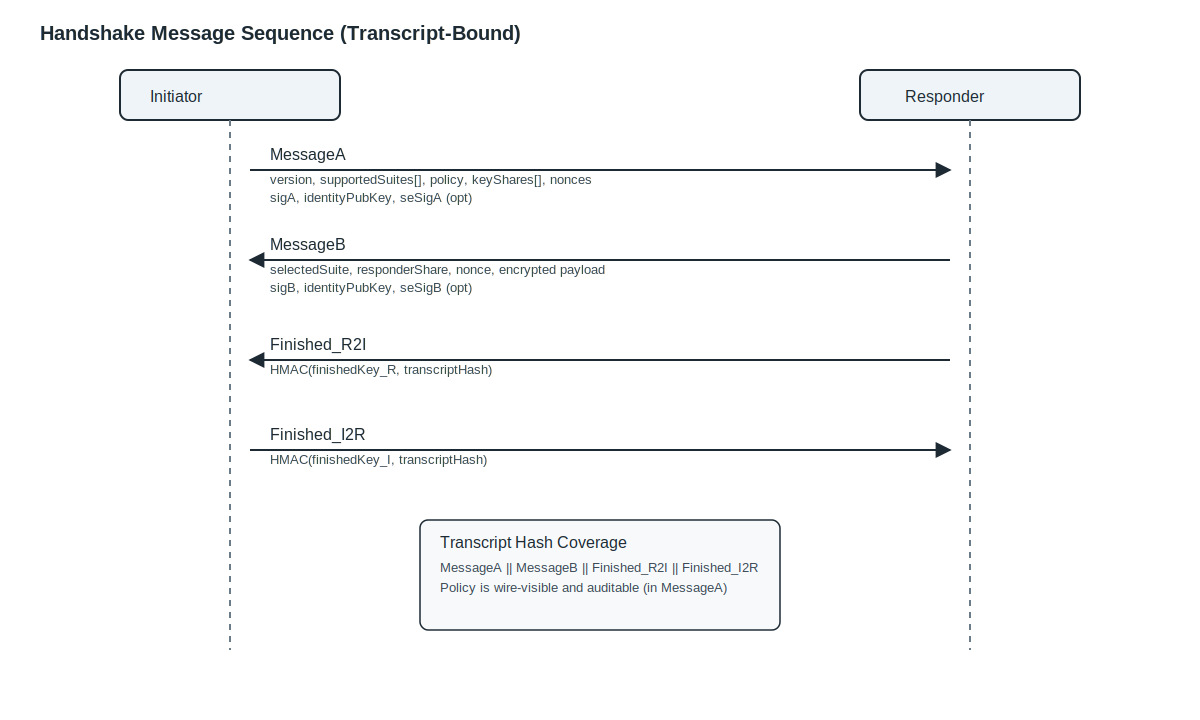
\includegraphics[keepaspectratio,width=\columnwidth]{figures/fig_handshake_sequence.png}}
\caption{Handshake sequence with transcript coverage and policy
visibility.}\label{fig:handshake-sequence}
\end{figure}

\textbf{Key Share Semantics:} The \texttt{keyShares{[}{]}.shareBytes}
field has suite-dependent interpretation: - \textbf{DH suites (X25519):}
\texttt{shareBytes} = ephemeral public key (32 bytes) - \textbf{KEM
suites (ML-KEM-768):} \texttt{shareBytes} = encapsulated key /
ciphertext (\texttt{enc}, 1088 bytes)

This distinction matters: for DH, the Responder uses the Initiator's
public key to compute a shared secret; for KEM, the Initiator has
already encapsulated to the Responder's long-term KEM public key
(obtained during pairing), and \texttt{shareBytes} carries the resulting
\texttt{enc}. The Responder decapsulates using their private key.

\textbf{Nonce Freshness:} Each party contributes a 32-byte nonce
(\texttt{clientNonce} in A, \texttt{serverNonce} in B). Both are bound
into the KDF info parameter, ensuring symmetric freshness and enabling a
unique session identifier:

\begin{quote}
\small\ttfamily
handshakeId = SHA256(replayTag\allowbreak\ || initiatorNonce\allowbreak\ || responderNonce\allowbreak\ || suiteWireIdLE)
\end{quote}

To prevent short-window replay attacks, implementations SHOULD cache
recent \texttt{handshakeId} values (or the
\texttt{(initiatorNonce,\ responderNonce)} pair) and reject duplicates
within a configurable window (default: 5 minutes).

\textbf{Key Share Binding:} The \texttt{keyShares{[}{]}} array contains
at most 2 entries (one PQC, one Classic) to bound message size while
enabling negotiation. Each entry is a \texttt{(suiteId,\ shareBytes)}
tuple. The Responder MUST select a suite for which the Initiator
provided a key share; otherwise reject with \texttt{missingKeyShare}.
This binds the negotiation to actual cryptographic material, preventing
the ``TLS key\_share mismatch'' class of bugs.

\textbf{Explicit Key Confirmation (Finished Frames):} Although the core
key schedule is derived after MessageB, SkyBridge Compass performs an
explicit key-confirmation exchange before entering the ``established''
state. The Responder sends a short \texttt{Finished\_R2I} frame
authenticated under the newly derived session keys; the Initiator
verifies it and replies with \texttt{Finished\_I2R}. A session is
considered established only after both Finished frames are verified.
This provides mutual key confirmation, eliminates ambiguity about the
establishment point, and reduces responder-side half-open state under
failures. The Finished frames are fixed-size authenticated messages (38
bytes each: 4-byte magic, 1-byte version, 1-byte direction, 32-byte
HMAC) and add negligible wire overhead compared to PQC handshake
payloads. The Finished MAC is computed as
\texttt{HMAC-SHA256(finishedKey,\ transcriptHash)} where
\texttt{finishedKey\ =\ HKDF(sessionKey,\ info="SkyBridge-FINISHED\textbar{}\textless{}role\textgreater{}\textbar{}")}.
Wire overhead for the full handshake including Finished frames is
reported in Table~\ref{tab:handshake-sizes}.

\textbf{Anti-Downgrade Invariant:} The Initiator MUST verify that
\texttt{selectedSuite} is a member of the \texttt{supportedSuites{[}{]}}
it originally sent AND that \texttt{keyShares{[}{]}} contains an entry
for \texttt{selectedSuite}. Since \texttt{sigB} commits to
\texttt{MessageA} (via \texttt{transcriptA}), any modification to
\texttt{supportedSuites{[}{]}} or \texttt{keyShares{[}{]}} by an
attacker will cause \texttt{sigB} verification to fail.

\textbf{Suite Negotiation Scenarios:}

\begin{table*}[!t]
\centering
\caption{Suite negotiation scenarios.}\label{tab:suite-negotiation}
\begin{tabular}{@{}
  >{\raggedright\arraybackslash}p{(\linewidth - 6\tabcolsep) * \real{0.4219}}
  >{\raggedright\arraybackslash}p{(\linewidth - 6\tabcolsep) * \real{0.3281}}
  >{\raggedright\arraybackslash}p{(\linewidth - 6\tabcolsep) * \real{0.1406}}
  >{\raggedright\arraybackslash}p{(\linewidth - 6\tabcolsep) * \real{0.1094}}@{}}
\toprule\noalign{}
\begin{minipage}[b]{\linewidth}\raggedright
Initiator supportedSuites
\end{minipage} & \begin{minipage}[b]{\linewidth}\raggedright
Responder Capability
\end{minipage} & \begin{minipage}[b]{\linewidth}\raggedright
Outcome
\end{minipage} & \begin{minipage}[b]{\linewidth}\raggedright
Notes
\end{minipage} \\
\midrule\noalign{}

\bottomrule\noalign{}

{[}PQC, Classic{]} & PQC available & PQC established & Best available
selected \\
{[}PQC, Classic{]} & Classic only & Classic established & Graceful
fallback \\
{[}PQC only{]} & Classic only & Handshake failed & Policy enforced \\
{[}Classic only{]} & PQC available & Classic established & Initiator
policy respected \\
\end{tabular}
\end{table*}

\textbf{Message Field Validation Rules:}

\begin{table*}[!t]
\centering
\caption{Message field validation rules.}\label{tab:message-validation}
\begin{tabular}{@{}
  >{\raggedright\arraybackslash}p{(\linewidth - 4\tabcolsep) * \real{0.2000}}
  >{\raggedright\arraybackslash}p{(\linewidth - 4\tabcolsep) * \real{0.3429}}
  >{\raggedright\arraybackslash}p{(\linewidth - 4\tabcolsep) * \real{0.4571}}@{}}
\toprule\noalign{}
\begin{minipage}[b]{\linewidth}\raggedright
Field
\end{minipage} & \begin{minipage}[b]{\linewidth}\raggedright
Validation
\end{minipage} & \begin{minipage}[b]{\linewidth}\raggedright
Failure Action
\end{minipage} \\
\midrule\noalign{}

\bottomrule\noalign{}

version & Must equal protocol version (1) & Reject with
versionMismatch \\
supportedSuites & Must contain at least one suite supported by local
implementation; unknown IDs are ignored for negotiation but still
transcript-bound & Reject with suiteNegotiationFailed \\
keyShares & Unique suiteId per entry, max 2 entries, each shareBytes
must match its suiteId's expected length & Reject with
invalidMessageFormat \\
selectedSuite & Must be in supportedSuites AND have matching keyShare &
Reject with missingKeyShare \\
clientNonce/serverNonce & Must be 32 bytes & Reject with
invalidMessageFormat \\
sigA/sigB & Must verify against respective identityPubKey & Reject with
signatureVerificationFailed \\
\end{tabular}
\end{table*}

\textbf{Canonical Encoding Rules:} - \texttt{supportedSuites{[}{]}}:
preference order, signed as-is (first = most preferred) -
\texttt{keyShares{[}{]}}: encoded in same order as
\texttt{supportedSuites{[}{]}} (only suites with provided shares) - All
lists use 2-byte little-endian length prefix - All integers use
little-endian encoding - Canonical encoding is byte-for-byte specified;
implementations MUST NOT reserialize with language-native encoders
(e.g., JSON, PropertyList) as this may introduce non-determinism

Note: The 32-byte \texttt{clientNonce}/\texttt{serverNonce} in message
fields are distinct from the 12-byte \texttt{aeadNonce} used internally
by AES-GCM for authenticated encryption.

\textbf{Failure Semantics:} - All failures trigger
\texttt{HandshakeContext.zeroize()} before error propagation - Security
events are emitted for audit logging - No partial state is retained
after failure

\begin{figure}
\centering
\resizebox{\columnwidth}{!}{%
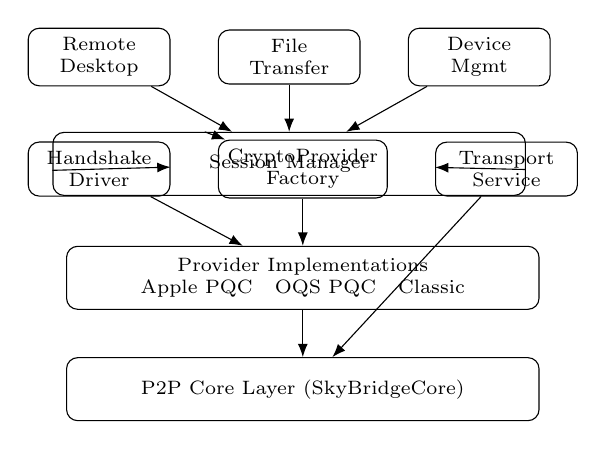
\begin{tikzpicture}[
  font=\scriptsize,
  box/.style={draw, rounded corners, align=center, minimum height=6mm, minimum width=18mm},
  layer/.style={draw, rounded corners, align=center, minimum height=8mm, minimum width=60mm},
  arrow/.style={-Latex, line width=0.4pt}
]
  % Top row
  \node[box] (rd) {Remote\\Desktop};
  \node[box, right=6mm of rd] (ft) {File\\Transfer};
  \node[box, right=6mm of ft] (dm) {Device\\Mgmt};

  % Session manager
  \node[layer, below=6mm of ft] (sm) {Session Manager};

  % Core services
  \node[box, below=7mm of rd] (hd) {Handshake\\Driver};
  \node[box, right=6mm of hd] (cpf) {CryptoProvider\\Factory};
  \node[box, right=6mm of cpf] (ts) {Transport\\Service};

  % Provider implementations
  \node[layer, below=6mm of cpf] (pi) {Provider Implementations\\Apple PQC\quad OQS PQC\quad Classic};

  % Core module
  \node[layer, below=6mm of pi] (core) {P2P Core Layer (SkyBridgeCore)};

  % Arrows
  \draw[arrow] (rd) -- (sm);
  \draw[arrow] (ft) -- (sm);
  \draw[arrow] (dm) -- (sm);

  \draw[arrow] (sm) -- (hd);
  \draw[arrow] (sm) -- (cpf);
  \draw[arrow] (sm) -- (ts);

  \draw[arrow] (cpf) -- (pi);
  \draw[arrow] (hd) -- (pi);
\draw[arrow] (ts) -- (core);
\draw[arrow] (pi) -- (core);
\end{tikzpicture}
}
\caption{SkyBridge Compass system architecture with trust boundaries and
policy guard.}\label{fig:architecture}
\end{figure}

\subsection{CryptoProvider
Protocol}\label{b.-cryptoprovider-protocol}

The CryptoProvider protocol defines a unified interface for all
cryptographic operations required by the handshake and session layers.
This abstraction enables transparent substitution of underlying
implementations without modifying caller code.

\begin{Shaded}
\begin{Highlighting}
\KeywordTok{public} \KeywordTok{protocol}\NormalTok{ CryptoProvider}\OperatorTok{:} \DataTypeTok{Sendable} \OperatorTok{\{}
    \KeywordTok{var} \VariableTok{providerName}\OperatorTok{:}\NormalTok{ String }\OperatorTok{\{} \KeywordTok{get} \OperatorTok{\}}
    \KeywordTok{var} \VariableTok{tier}\OperatorTok{:}\NormalTok{ CryptoTier }\OperatorTok{\{} \KeywordTok{get} \OperatorTok{\}}
    \KeywordTok{var} \VariableTok{activeSuite}\OperatorTok{:}\NormalTok{ CryptoSuite }\OperatorTok{\{} \KeywordTok{get} \OperatorTok{\}}
    
    \KeywordTok{func} \FunctionTok{kemDemSeal}\OperatorTok{(}\VariableTok{plaintext}\OperatorTok{:} \DataTypeTok{Data}\OperatorTok{,} \VariableTok{recipientPublicKey}\OperatorTok{:} \DataTypeTok{Data}\OperatorTok{,} 
                    \VariableTok{info}\OperatorTok{:} \DataTypeTok{Data}\OperatorTok{)} \FunctionTok{async} \KeywordTok{throws}\NormalTok{ {-}\textgreater{} }\FunctionTok{KemDemSealedBox}
    \KeywordTok{func} \FunctionTok{kemDemOpen}\OperatorTok{(}\VariableTok{sealedBox}\OperatorTok{:} \DataTypeTok{KemDemSealedBox}\OperatorTok{,} \VariableTok{privateKey}\OperatorTok{:} \DataTypeTok{Data}\OperatorTok{,} 
                    \VariableTok{info}\OperatorTok{:} \DataTypeTok{Data}\OperatorTok{)} \FunctionTok{async} \KeywordTok{throws}\NormalTok{ {-}\textgreater{} }\FunctionTok{Data}
    \KeywordTok{func} \FunctionTok{sign}\OperatorTok{(}\VariableTok{data}\OperatorTok{:} \DataTypeTok{Data}\OperatorTok{,} \VariableTok{using} \VariableTok{key}\OperatorTok{:} \DataTypeTok{SigningKeyHandle}\OperatorTok{)} \FunctionTok{async} \KeywordTok{throws}\NormalTok{ {-}\textgreater{} }\FunctionTok{Data}
    \KeywordTok{func} \FunctionTok{verify}\OperatorTok{(}\VariableTok{data}\OperatorTok{:} \DataTypeTok{Data}\OperatorTok{,} \VariableTok{signature}\OperatorTok{:} \DataTypeTok{Data}\OperatorTok{,} 
                \VariableTok{publicKey}\OperatorTok{:} \DataTypeTok{Data}\OperatorTok{)} \FunctionTok{async} \KeywordTok{throws}\NormalTok{ {-}\textgreater{} }\FunctionTok{Bool}
    \KeywordTok{func} \FunctionTok{generateKeyPair}\OperatorTok{(}\VariableTok{for} \VariableTok{usage}\OperatorTok{:} \DataTypeTok{KeyUsage}\OperatorTok{)} \FunctionTok{async} \KeywordTok{throws}\NormalTok{ {-}\textgreater{} }\FunctionTok{KeyPair}
\OperatorTok{\}}

\CommentTok{/// Abstraction for signing keys: software or hardware{-}backed}
\KeywordTok{public} \KeywordTok{enum}\NormalTok{ SigningKeyHandle}\OperatorTok{:} \DataTypeTok{Sendable} \OperatorTok{\{}
    \ControlFlowTok{case}\NormalTok{ softwareKey}\OperatorTok{(}\NormalTok{Data}\OperatorTok{)}                    \CommentTok{// Exportable private key bytes}
    \ControlFlowTok{case}\NormalTok{ secureEnclaveRef}\OperatorTok{(}\NormalTok{SecKey}\OperatorTok{)}             \CommentTok{// Hardware{-}backed, non{-}exportable}
    \ControlFlowTok{case}\NormalTok{ callback}\OperatorTok{(}\NormalTok{any SigningCallback}\OperatorTok{)}        \CommentTok{// Delegate to external signer}
\OperatorTok{\}}
\end{Highlighting}
\end{Shaded}

The \texttt{SigningKeyHandle} abstraction resolves the apparent conflict
between ``private key as Data'' and ``Secure Enclave keys never leave
hardware.'' Software keys are one variant; hardware-backed keys use a
reference or callback, ensuring the protocol interface does not assume
exportability.

The protocol mandates \texttt{Sendable} conformance, ensuring
thread-safe usage across Swift's structured concurrency model. Each
provider exposes its tier classification (\texttt{nativePQC},
\texttt{liboqsPQC}, or \texttt{classic}) and active cipher suite,
enabling runtime introspection for logging and policy enforcement.

\subsection{CryptoSuite Wire
Format}\label{c.-cryptosuite-wire-format}

A \textbf{suite} defines the complete tuple
\texttt{(KEM,\ SIG,\ AEAD,\ KDF)}. Algorithm suite identifiers use a
structured 16-bit wire format enabling forward compatibility:

\begin{table*}[!t]
\centering
\caption{Suite identifier ranges and components.}\label{tab:suite-identifiers}
\begin{tabular}{@{}
  >{\raggedright\arraybackslash}p{(\linewidth - 6\tabcolsep) * \real{0.1556}}
  >{\raggedright\arraybackslash}p{(\linewidth - 6\tabcolsep) * \real{0.2222}}
  >{\raggedright\arraybackslash}p{(\linewidth - 6\tabcolsep) * \real{0.4000}}
  >{\raggedright\arraybackslash}p{(\linewidth - 6\tabcolsep) * \real{0.2222}}@{}}
\toprule\noalign{}
\begin{minipage}[b]{\linewidth}\raggedright
Range
\end{minipage} & \begin{minipage}[b]{\linewidth}\raggedright
Category
\end{minipage} & \begin{minipage}[b]{\linewidth}\raggedright
Suite Components
\end{minipage} & \begin{minipage}[b]{\linewidth}\raggedright
Examples
\end{minipage} \\
\midrule\noalign{}

\bottomrule\noalign{}

0x00xx & Hybrid PQC (preferred) & X-Wing KEM, ML-DSA-65, AES-256-GCM,
HKDF-SHA256 & 0x0001 \\
0x01xx & Pure PQC & ML-KEM-768, ML-DSA-65, AES-256-GCM, HKDF-SHA256 &
0x0101 \\
0x10xx & Classic & X25519 DHKEM, Ed25519, AES-256-GCM, HKDF-SHA256 &
0x1001 \\
0xF0xx & Experimental & Reserved for testing & - \\
\end{tabular}
\end{table*}

Note: X-Wing is a hybrid KEM combining X25519 + ML-KEM-768; it does not
include a signature algorithm. The suite identifier specifies the full
primitive set, with ML-DSA-65 as the \emph{preferred} signature
algorithm when available; the current implementation may fall back to
classic signatures (Ed25519 / Secure Enclave P-256) for broader
OS/toolchain compatibility while keeping PQC confidentiality.

Unknown suite identifiers are parsed as \texttt{unknown(wireId)} rather
than causing parse failures, allowing older clients to gracefully reject
unsupported suites during negotiation.

\subsection{Provider Factory and
Selection}\label{d.-provider-factory-and-selection}

The \texttt{CryptoProviderFactory} implements deterministic provider
selection based on runtime capability detection and policy
configuration:

\begin{Shaded}
\begin{Highlighting}
\KeywordTok{public} \KeywordTok{enum}\NormalTok{ CryptoProviderFactory }\OperatorTok{\{}
    \KeywordTok{public} \KeywordTok{enum}\NormalTok{ SelectionPolicy}\OperatorTok{:} \DataTypeTok{Sendable} \OperatorTok{\{}
        \ControlFlowTok{case}\NormalTok{ preferPQC      }\CommentTok{// Default: best available}
        \ControlFlowTok{case}\NormalTok{ requirePQC     }\CommentTok{// Fail if PQC unavailable}
        \ControlFlowTok{case}\NormalTok{ classicOnly    }\CommentTok{// Force classic algorithms}
    \OperatorTok{\}}
    
    \KeywordTok{public} \KeywordTok{static} \KeywordTok{func} \FunctionTok{make}\OperatorTok{(}
        \VariableTok{policy}\OperatorTok{:} \DataTypeTok{SelectionPolicy} \OperatorTok{=} \OperatorTok{.}\NormalTok{preferPQC}\OperatorTok{,}
        \VariableTok{environment}\OperatorTok{:} \DataTypeTok{any} \VariableTok{CryptoEnvironment} \OperatorTok{=}\NormalTok{ SystemCryptoEnvironment}\OperatorTok{.}\NormalTok{system}
    \OperatorTok{)}\NormalTok{ {-}\textgreater{} }\FunctionTok{any} \FunctionTok{CryptoProvider}
\OperatorTok{\}}
\end{Highlighting}
\end{Shaded}

The selection algorithm proceeds as follows:

\begin{enumerate}
\def\labelenumi{\arabic{enumi}.}
\tightlist
\item
  \textbf{Capability Detection:} Query the environment for Apple PQC
  availability (macOS 26+) and liboqs presence.
\item
  \textbf{Policy Application:} Match detected capabilities against the
  requested policy.
\item
  \textbf{Provider Instantiation:} Create the appropriate provider
  instance.
\item
  \textbf{Event Emission:} Emit a \texttt{SecurityEvent} recording the
  selection decision.
\end{enumerate}

For \texttt{preferPQC} policy, the precedence order is: ApplePQCProvider
-\textgreater{} OQSPQCProvider -\textgreater{} ClassicProvider. The
\texttt{requirePQC} policy returns an \texttt{UnavailablePQCProvider}
that throws on all operations if no PQC implementation is available.

\subsection{KEM-DEM Authenticated Encryption
Format}\label{e.-kem-dem-authenticated-encryption-format}

The sealed box structure encapsulates KEM-based authenticated encryption
output with explicit DoS protection. Our construction follows the
KEM-DEM (Key Encapsulation Mechanism + Data Encapsulation Mechanism)
paradigm: KEM.Encapsulate() -\textgreater{} HKDF-SHA256 -\textgreater{}
AES-256-GCM. We call this an ``HPKE-inspired KEM-DEM envelope'' to
distinguish it from RFC 9180 HPKE \cite{ref13}, which includes additional
features such as multiple modes (Base, PSK, Auth, AuthPSK), context
exporters, and a more complex key schedule.

On Apple 26+ platforms, CryptoKit provides native HPKE with
quantum-secure cipher suites including X-Wing (ML-KEM-768 + X25519)
\cite{ref14}. When available, implementations SHOULD use CryptoKit's HPKE
API directly rather than this compatibility envelope.

\textbf{Security Goals:} - PQC suites: ML-KEM provides IND-CCA2 KEM
security (per FIPS 203) - Classic suites: X25519 ephemeral-DH
encapsulation (DHKEM-style); security relies on the X25519/Gap-DH
assumption and HKDF key separation - INT-CTXT and IND-CPA for the
payload encryption: AES-256-GCM in v1 (compat KEM-DEM), and RFC 9180
HPKE AEAD in v2 (e.g., ChaCha20-Poly1305 in our classic provider) - Key
separation via HKDF with context-specific info parameters including role
binding

\textbf{Not Covered (delegated to RFC 9180 HPKE on Apple 26+):} - Sender
authentication modes (Auth, AuthPSK) - Incremental AEAD for streaming

\textbf{Used in our handshake (classic v2):} - HPKE exporter for
deriving the per-session shared secret with explicit context binding

\textbf{Format Versions:}

The implementation supports two sealed box formats:

\textbf{v1 (Compatibility KEM-DEM):} Used when native HPKE is
unavailable. Explicit nonce and tag fields.

Header (17 bytes):
\begin{center}
\small
\begin{tabular}{|c|c|c|c|}
\hline
magic & version & suite & flags \\
\hline
4B & 1B & 2B & 2B \\
\hline
encLen & nonceLen & tagLen & ctLen \\
\hline
2B & 1B & 1B & 4B \\
\hline
\end{tabular}
\end{center}

Body (v1):
\begin{center}
\small
\begin{tabular}{|c|c|c|c|}
\hline
encapsulatedKey & nonce & ciphertext & tag \\
\hline
encLen & 12B & ctLen & 16B \\
\hline
\end{tabular}
\end{center}

\textbf{v2 (Native HPKE):} Used with CryptoKit HPKE. Nonce and tag are
embedded in the AEAD output.

Header (17 bytes):
\begin{center}
\small
\begin{tabular}{|c|c|c|c|}
\hline
magic & version & suite & flags \\
\hline
4B & 1B & 2B & 2B \\
\hline
encLen & nonceLen & tagLen & ctLen \\
\hline
2B & 0 & 0 & 4B \\
\hline
\end{tabular}
\end{center}

Body (v2):
\begin{center}
\small
\begin{tabular}{|c|c|}
\hline
encapsulatedKey & ciphertext (AEAD output) \\
\hline
encLen & ctLen (includes auth tag) \\
\hline
\end{tabular}
\end{center}

\textbf{Version Detection:} Parsers distinguish v1 from v2 by checking
\texttt{nonceLen} and \texttt{tagLen}: - v1: \texttt{nonceLen\ =\ 12},
\texttt{tagLen\ =\ 16} - v2: \texttt{nonceLen\ =\ 0},
\texttt{tagLen\ =\ 0} (AEAD details encapsulated by library)

Length limits enforce DoS protection: - \texttt{encLen} \textless= 4096
bytes (sufficient for ML-KEM-768's 1088-byte ciphertext) - v1:
\texttt{nonceLen} = 12 bytes (AES-GCM fixed), \texttt{tagLen} = 16 bytes
(AES-GCM fixed) - v2: \texttt{nonceLen} = 0, \texttt{tagLen} = 0
(embedded in ciphertext) - \texttt{ctLen} \textless= 64KB (handshake
phase, pre-authentication) or 256KB (post-authentication)

Parsing uses overflow-safe arithmetic and validates each field before
allocation.



\section{HANDSHAKE STATE
MACHINE}\label{iv.-handshake-state-machine}

\subsection{Design Principles}\label{a.-design-principles}

The handshake subsystem addresses three critical requirements:

\begin{enumerate}
\def\labelenumi{\arabic{enumi}.}
\tightlist
\item
  \textbf{Race Condition Prevention:} Concurrent message arrival and
  timeout expiration must not cause double-resume of continuations.
\item
  \textbf{Sensitive Material Protection:} Ephemeral private keys and
  shared secrets must be zeroized on all exit paths.
\item
  \textbf{Observability:} All state transitions and failures must emit
  structured events.
\end{enumerate}

\subsection{Actor-Isolated
Architecture}\label{b.-actor-isolated-architecture}

The \texttt{HandshakeDriver} actor manages handshake state with
compile-time data race prevention:

\begin{Shaded}
\begin{Highlighting}
\KeywordTok{public} \ControlFlowTok{actor}\NormalTok{ HandshakeDriver }\OperatorTok{\{}
    \KeywordTok{private} \KeywordTok{var} \VariableTok{state}\OperatorTok{:}\NormalTok{ HandshakeState }\OperatorTok{=} \OperatorTok{.}\NormalTok{idle}
    \KeywordTok{private} \KeywordTok{var} \VariableTok{pendingContinuation}\OperatorTok{:}\NormalTok{ CheckedContinuation}\OperatorTok{\textless{}}\NormalTok{SessionKeys}\OperatorTok{,}\NormalTok{ Error}\OperatorTok{\textgreater{}?}
    \KeywordTok{private} \KeywordTok{var} \VariableTok{timeoutTask}\OperatorTok{:}\NormalTok{ Task}\OperatorTok{\textless{}}\NormalTok{Void}\OperatorTok{,}\NormalTok{ Never}\OperatorTok{\textgreater{}?}
    \KeywordTok{private} \KeywordTok{var} \VariableTok{pendingResult}\OperatorTok{:}\NormalTok{ Result}\OperatorTok{\textless{}}\NormalTok{SessionKeys}\OperatorTok{,}\NormalTok{ Error}\OperatorTok{\textgreater{}?}
    
    \KeywordTok{public} \KeywordTok{func} \FunctionTok{initiateHandshake}\OperatorTok{(}\VariableTok{with} \VariableTok{peer}\OperatorTok{:} \DataTypeTok{PeerIdentifier}\OperatorTok{)} 
        \FunctionTok{async} \KeywordTok{throws}\NormalTok{ {-}\textgreater{} }\FunctionTok{SessionKeys}
    \KeywordTok{public} \KeywordTok{func} \FunctionTok{handleMessage}\OperatorTok{(}\VariableTok{\_} \VariableTok{data}\OperatorTok{:} \DataTypeTok{Data}\OperatorTok{,} \VariableTok{from} \VariableTok{peer}\OperatorTok{:} \DataTypeTok{PeerIdentifier}\OperatorTok{)} \FunctionTok{async}
    \KeywordTok{public} \KeywordTok{func} \FunctionTok{cancel}\OperatorTok{()} \FunctionTok{async}
\OperatorTok{\}}
\end{Highlighting}
\end{Shaded}

The \texttt{HandshakeContext} actor isolates sensitive cryptographic
material:

\begin{Shaded}
\begin{Highlighting}
\KeywordTok{public} \ControlFlowTok{actor}\NormalTok{ HandshakeContext }\OperatorTok{\{}
    \KeywordTok{private} \KeywordTok{var} \VariableTok{ephemeralPrivateKey}\OperatorTok{:}\NormalTok{ SecureBytes}\OperatorTok{?}
    \KeywordTok{private} \KeywordTok{var} \VariableTok{transcriptHash}\OperatorTok{:}\NormalTok{ SecureBytes}\OperatorTok{?}
    \KeywordTok{private} \KeywordTok{var} \VariableTok{isZeroized}\OperatorTok{:}\NormalTok{ Bool }\OperatorTok{=} \KeywordTok{false}
    
    \KeywordTok{public} \KeywordTok{func} \FunctionTok{zeroize}\OperatorTok{()}
\OperatorTok{\}}
\end{Highlighting}
\end{Shaded}

\textbf{Reentrancy Considerations.} Swift actors permit method re-entry
at suspension points (\texttt{await}). While actor isolation prevents
data races, it does not prevent interleaving of method executions. Our
\texttt{HandshakeDriver} mitigates reentrancy risks through several
mechanisms:

\begin{enumerate}
\def\labelenumi{\arabic{enumi}.}
\item
  \textbf{Single convergence point:} The \texttt{finishOnce(with:)}
  method provides a single point for handshake completion. It guards
  \texttt{pendingContinuation} access and immediately sets the reference
  to \texttt{nil} after resume, preventing double-resume even if called
  concurrently from timeout and message handlers.
\item
  \textbf{Early result buffering:} The \texttt{pendingResult} property
  stores results that arrive before the continuation is established
  (e.g., if \texttt{MessageB} arrives before
  \texttt{withCheckedThrowingContinuation} captures the continuation).
\item
  \textbf{Timeout cancellation:} \texttt{timeoutTask} is cancelled in
  \texttt{finishOnce}, preventing the race between timeout expiration
  and successful message receipt.
\item
  \textbf{State advancement:} State transitions occur before
  \texttt{await} points where possible, reducing the window for
  interleaved operations.
\end{enumerate}

\textbf{Acknowledged Limitation:} The \texttt{handleMessageB} method
awaits \texttt{cryptoProvider} operations inside the actor. If a new
message arrives during this await, the actor could theoretically process
it before the current operation completes. We mitigate this structurally
by: - Advancing state to \texttt{.processingMessageB} before the await,
causing subsequent messages to be rejected or queued - Copying all
necessary immutable inputs before the await point - Validating a
monotonic epoch counter after the await returns, ensuring the actor
state has not been invalidated by concurrent operations - Emitting
security events for any unexpected state transitions

This approach provides structural guarantees against reentrancy hazards
rather than relying on timing assumptions. A formal analysis using model
checking is planned for future work.

\subsection{State Transitions}\label{c.-state-transitions}

Fig.~\ref{fig:handshake-state-machine} illustrates the handshake state
machine for both roles.

\begin{figure}
\centering
\pandocbounded{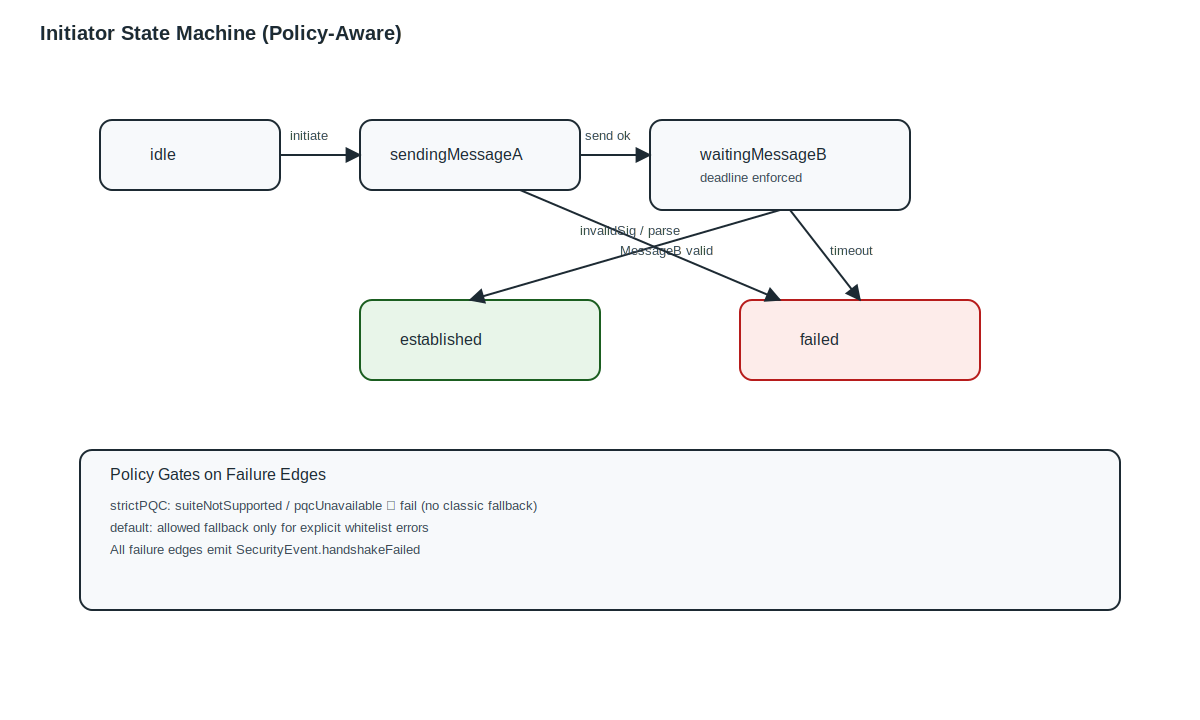
\includegraphics[keepaspectratio,width=\columnwidth]{figures/fig_state_machine_initiator.png}}
\vspace{2mm}
\pandocbounded{\includegraphics[keepaspectratio,width=\columnwidth]{figures/fig_state_machine_responder.png}}
\caption{Handshake state machines for Initiator (top) and Responder
(bottom).}\label{fig:handshake-state-machine}
\end{figure}

\subsection{Double-Resume
Prevention}\label{d.-double-resume-prevention}

The \texttt{finishOnce} method provides a single convergence point for
handshake completion:

\begin{Shaded}
\begin{Highlighting}
\KeywordTok{private} \KeywordTok{func} \FunctionTok{finishOnce}\OperatorTok{(}\VariableTok{with} \VariableTok{result}\OperatorTok{:} \DataTypeTok{Result}\NormalTok{\textless{}}\VariableTok{SessionKeys}\OperatorTok{,} \VariableTok{Error}\NormalTok{\textgreater{}}\OperatorTok{)} \OperatorTok{\{}
    \CommentTok{// Cancel timeout}
\NormalTok{    timeoutTask}\OperatorTok{?.}\NormalTok{cancel}\OperatorTok{()}
\NormalTok{    timeoutTask }\OperatorTok{=} \KeywordTok{nil}
    
    \CommentTok{// Guard against double resume}
    \ControlFlowTok{guard} \KeywordTok{let} \VariableTok{continuation} \OperatorTok{=}\NormalTok{ pendingContinuation }\ControlFlowTok{else} \OperatorTok{\{}
        \CommentTok{// MessageB arrived before continuation established}
\NormalTok{        pendingResult }\OperatorTok{=}\NormalTok{ result}
        \KeywordTok{return}
    \OperatorTok{\}}
\NormalTok{    pendingContinuation }\OperatorTok{=} \KeywordTok{nil}  \CommentTok{// Immediately nil to prevent reuse}
    
    \ControlFlowTok{switch}\NormalTok{ result }\OperatorTok{\{}
    \ControlFlowTok{case} \OperatorTok{.}\NormalTok{success}\OperatorTok{(}\KeywordTok{let} \VariableTok{keys}\OperatorTok{):}\NormalTok{ continuation}\OperatorTok{.}\NormalTok{resume}\OperatorTok{(}\NormalTok{returning}\OperatorTok{:}\NormalTok{ keys}\OperatorTok{)}
    \ControlFlowTok{case} \OperatorTok{.}\NormalTok{failure}\OperatorTok{(}\KeywordTok{let} \VariableTok{error}\OperatorTok{):}\NormalTok{ continuation}\OperatorTok{.}\NormalTok{resume}\OperatorTok{(}\NormalTok{throwing}\OperatorTok{:}\NormalTok{ error}\OperatorTok{)}
    \OperatorTok{\}}
\OperatorTok{\}}
\end{Highlighting}
\end{Shaded}

This pattern handles the race between timeout expiration and message
arrival by: 1. Canceling the timeout task on any completion 2. Guarding
continuation access with immediate nil assignment 3. Buffering early
results in \texttt{pendingResult} for late continuation establishment

\subsection{Secure Zeroization}\label{e.-secure-zeroization}

Swift's standard \texttt{Data} and \texttt{Array} types use
copy-on-write (COW) semantics, which can leave uncontrolled copies of
sensitive material in memory. The \texttt{SecureBytes} class addresses
this by using manual \texttt{UnsafeMutableRawPointer} allocation to
maintain exclusive ownership of the memory region, preventing
COW-induced secret proliferation.

\begin{Shaded}
\begin{Highlighting}
\KeywordTok{public} \KeywordTok{final} \KeywordTok{class}\NormalTok{ SecureBytes}\OperatorTok{:} \AttributeTok{@unchecked}\NormalTok{ Sendable }\OperatorTok{\{}
    \KeywordTok{private} \KeywordTok{let} \VariableTok{pointer}\OperatorTok{:}\NormalTok{ UnsafeMutableRawPointer}
    \KeywordTok{private} \KeywordTok{let} \VariableTok{count}\OperatorTok{:}\NormalTok{ Int}
    
    \CommentTok{/// Injectable wiping function for test verification}
\NormalTok{    nonisolated}\OperatorTok{(}\NormalTok{unsafe}\OperatorTok{)} \KeywordTok{public} \KeywordTok{static} \KeywordTok{var} \VariableTok{wipingFunction}\OperatorTok{:} 
        \OperatorTok{(}\NormalTok{UnsafeMutableRawPointer}\OperatorTok{,}\NormalTok{ Int}\OperatorTok{)} \OperatorTok{{-}\textgreater{}}\NormalTok{ Void }\OperatorTok{=}\NormalTok{ secureZero}
    
    \KeywordTok{deinit} \OperatorTok{\{}
        \ControlFlowTok{if}\NormalTok{ count }\OperatorTok{\textgreater{}} \DecValTok{0} \OperatorTok{\{}
\NormalTok{            Self}\OperatorTok{.}\NormalTok{wipingFunction}\OperatorTok{(}\NormalTok{pointer}\OperatorTok{,}\NormalTok{ count}\OperatorTok{)}
        \OperatorTok{\}}
\NormalTok{        pointer}\OperatorTok{.}\NormalTok{deallocate}\OperatorTok{()}
    \OperatorTok{\}}
\OperatorTok{\}}
\end{Highlighting}
\end{Shaded}

\textbf{Design Rationale:}

\begin{enumerate}
\def\labelenumi{\arabic{enumi}.}
\item
  \textbf{Avoiding Copy-on-Write:} The primary motivation for
  \texttt{SecureBytes} is to prevent COW semantics from creating
  untracked copies of ephemeral keys and shared secrets. All sensitive
  material in \texttt{HandshakeContext} uses \texttt{SecureBytes} rather
  than \texttt{Data}.
\item
  \textbf{Explicit Zeroization on Failure Paths:} Because Swift's ARC
  does not guarantee \texttt{deinit} timing, all failure paths in
  \texttt{HandshakeDriver} explicitly call \texttt{context.zeroize()}
  before error propagation. The \texttt{deinit} zeroization serves as a
  defense-in-depth fallback, not the primary mechanism.
\item
  \textbf{Compiler Optimization Resistance:} On Darwin platforms,
  zeroization uses platform-supported secure wipe primitives where
  available, or \texttt{memset} followed by
  \texttt{withExtendedLifetime} as a fallback. We aim for best-effort
  zeroization; complete guarantees depend on compiler/runtime semantics
  and are not formally provable in Swift today.
\item
  \textbf{Test Verification:} The \texttt{wipingFunction} is a static
  property that can be replaced during testing. This enables
  verification that zeroization paths are exercised on all failure
  modes, as demonstrated in Section VII.B.1.
\end{enumerate}

\subsection{Transcript Binding and Signature
Separation}\label{f.-transcript-binding-and-signature-separation}

The protocol uses domain-separated signatures to prevent cross-message
and cross-session replay attacks.

\textbf{Signature A (MessageA):} The Initiator signs only MessageA-local
fields:

\begin{Shaded}
\begin{Highlighting}
\CommentTok{// preimageA: fields known to Initiator at MessageA time}
\KeywordTok{let} \VariableTok{preimageA} \OperatorTok{=}\NormalTok{ Data}\OperatorTok{()}
    \OperatorTok{+}\NormalTok{ DS}\OperatorTok{(}\StringTok{"SkyBridge{-}A"}\OperatorTok{)}                           \CommentTok{// Domain separator}
    \OperatorTok{+}\NormalTok{ version}\OperatorTok{.}\NormalTok{encoded}
    \OperatorTok{+}\NormalTok{ supportedSuites}\OperatorTok{.}\NormalTok{canonicalEncode}\OperatorTok{()}           \CommentTok{// Preference order preserved}
    \OperatorTok{+}\NormalTok{ keyShares}\OperatorTok{.}\NormalTok{canonicalEncode}\OperatorTok{()}                 \CommentTok{// Bound to supportedSuites order}
    \OperatorTok{+}\NormalTok{ clientNonce                                 }\CommentTok{// 32 bytes}
    \OperatorTok{+}\NormalTok{ capabilities}\OperatorTok{.}\NormalTok{canonicalEncode}\OperatorTok{()}
    \OperatorTok{+}\NormalTok{ policy}\OperatorTok{.}\NormalTok{canonicalEncode}\OperatorTok{()}
    \OperatorTok{+}\NormalTok{ identityPubKey\_I}

\NormalTok{sigA }\OperatorTok{=}\NormalTok{ Sign}\OperatorTok{(}\NormalTok{preimageA}\OperatorTok{,}\NormalTok{ identityPrivKey\_I}\OperatorTok{)}

\CommentTok{// Optional Secure Enclave binding (prevents SE proof replay)}
\NormalTok{seSigA }\OperatorTok{=}\NormalTok{ SE\_Sign}\OperatorTok{(}\NormalTok{DS}\OperatorTok{(}\StringTok{"SkyBridge{-}SE{-}A"}\OperatorTok{)} \OperatorTok{||}\NormalTok{ SHA256}\OperatorTok{(}\NormalTok{preimageA}\OperatorTok{))}
\end{Highlighting}
\end{Shaded}

\textbf{Signature B (MessageB):} The Responder signs a transcript that
commits to MessageA:

\begin{Shaded}
\begin{Highlighting}
\CommentTok{// transcriptA: hash of MessageA (excluding sigA and seSigA)}
\KeywordTok{let} \VariableTok{transcriptA} \OperatorTok{=}\NormalTok{ SHA256}\OperatorTok{(}\NormalTok{MessageA\_without\_signatures}\OperatorTok{)}

\KeywordTok{let} \VariableTok{preimageB} \OperatorTok{=}\NormalTok{ Data}\OperatorTok{()}
    \OperatorTok{+}\NormalTok{ DS}\OperatorTok{(}\StringTok{"SkyBridge{-}B"}\OperatorTok{)}                           \CommentTok{// Domain separator}
    \OperatorTok{+}\NormalTok{ transcriptA                                 }\CommentTok{// Commits to entire MessageA}
    \OperatorTok{+}\NormalTok{ selectedSuite}\OperatorTok{.}\NormalTok{wireId}\OperatorTok{.}\NormalTok{encoded}
    \OperatorTok{+}\NormalTok{ responderEphPubKey}
    \OperatorTok{+}\NormalTok{ serverNonce                                 }\CommentTok{// 32 bytes, fresh}
    \OperatorTok{+}\NormalTok{ SHA256}\OperatorTok{(}\NormalTok{encryptedPayload}\OperatorTok{)}                    \CommentTok{// Bind payload without bloating sig}
    \OperatorTok{+}\NormalTok{ identityPubKey\_R}

\NormalTok{sigB }\OperatorTok{=}\NormalTok{ Sign}\OperatorTok{(}\NormalTok{preimageB}\OperatorTok{,}\NormalTok{ identityPrivKey\_R}\OperatorTok{)}

\CommentTok{// Optional Secure Enclave binding}
\NormalTok{seSigB }\OperatorTok{=}\NormalTok{ SE\_Sign}\OperatorTok{(}\NormalTok{DS}\OperatorTok{(}\StringTok{"SkyBridge{-}SE{-}B"}\OperatorTok{)} \OperatorTok{||}\NormalTok{ SHA256}\OperatorTok{(}\NormalTok{preimageB}\OperatorTok{))}
\end{Highlighting}
\end{Shaded}

\textbf{Key Derivation:} Nonces, transcripts, suite binding, and
\emph{directional separation} are included in the KDF, and the salt is
transcript-bound (non-empty):

\begin{Shaded}
\begin{Highlighting}
\KeywordTok{let} \VariableTok{kdfInfo} \OperatorTok{=}\NormalTok{ Data}\OperatorTok{()}
    \OperatorTok{+}\NormalTok{ DS}\OperatorTok{(}\StringTok{"SkyBridge{-}KDF"}\OperatorTok{)}
    \OperatorTok{+}\NormalTok{ selectedSuite}\OperatorTok{.}\NormalTok{wireId}\OperatorTok{.}\NormalTok{encodedLE}
    \OperatorTok{+}\NormalTok{ transcriptA}
    \OperatorTok{+}\NormalTok{ transcriptB                      }\CommentTok{// e.g., SHA256(MessageB\_without\_signatures)}
    \OperatorTok{+}\NormalTok{ clientNonce}
    \OperatorTok{+}\NormalTok{ serverNonce}

\CommentTok{// Transcript{-}bound salt (prevents cross{-}context reuse)}
\KeywordTok{let} \VariableTok{salt} \OperatorTok{=}\NormalTok{ SHA256}\OperatorTok{(}\NormalTok{DS}\OperatorTok{(}\StringTok{"SkyBridge{-}KDF{-}Salt{-}v1|"}\OperatorTok{)} \OperatorTok{||}\NormalTok{ kdfInfo}\OperatorTok{)}

\CommentTok{// Direction{-}based symmetric key derivation}
\CommentTok{// Both sides derive the same key for each direction:}
\CommentTok{// {-} initiator\_to\_responder: Initiator\textquotesingle{}s sendKey = Responder\textquotesingle{}s receiveKey}
\CommentTok{// {-} responder\_to\_initiator: Responder\textquotesingle{}s sendKey = Initiator\textquotesingle{}s receiveKey}
\KeywordTok{let} \VariableTok{i2rInfo} \OperatorTok{=}\NormalTok{ kdfInfo }\OperatorTok{+}\NormalTok{ DS}\OperatorTok{(}\StringTok{"handshake|initiator\_to\_responder"}\OperatorTok{)}
\KeywordTok{let} \VariableTok{r2iInfo} \OperatorTok{=}\NormalTok{ kdfInfo }\OperatorTok{+}\NormalTok{ DS}\OperatorTok{(}\StringTok{"handshake|responder\_to\_initiator"}\OperatorTok{)}

\CommentTok{// For Initiator: sendKey = I2R, receiveKey = R2I}
\CommentTok{// For Responder: sendKey = R2I, receiveKey = I2R}
\KeywordTok{let} \VariableTok{sendKey} \OperatorTok{=}\NormalTok{ HKDF}\OperatorTok{\textless{}}\NormalTok{SHA256}\OperatorTok{\textgreater{}.}\NormalTok{deriveKey}\OperatorTok{(}
\NormalTok{    inputKeyMaterial}\OperatorTok{:}\NormalTok{ sharedSecret}\OperatorTok{,}
\NormalTok{    salt}\OperatorTok{:}\NormalTok{ salt}\OperatorTok{,}
\NormalTok{    info}\OperatorTok{:}\NormalTok{ role }\OperatorTok{==} \OperatorTok{.}\NormalTok{initiator }\OperatorTok{?}\NormalTok{ i2rInfo }\OperatorTok{:}\NormalTok{ r2iInfo}\OperatorTok{,}
\NormalTok{    outputByteCount}\OperatorTok{:} \DecValTok{32}
\OperatorTok{)}

\KeywordTok{let} \VariableTok{receiveKey} \OperatorTok{=}\NormalTok{ HKDF}\OperatorTok{\textless{}}\NormalTok{SHA256}\OperatorTok{\textgreater{}.}\NormalTok{deriveKey}\OperatorTok{(}
\NormalTok{    inputKeyMaterial}\OperatorTok{:}\NormalTok{ sharedSecret}\OperatorTok{,}
\NormalTok{    salt}\OperatorTok{:}\NormalTok{ salt}\OperatorTok{,}
\NormalTok{    info}\OperatorTok{:}\NormalTok{ role }\OperatorTok{==} \OperatorTok{.}\NormalTok{initiator }\OperatorTok{?}\NormalTok{ r2iInfo }\OperatorTok{:}\NormalTok{ i2rInfo}\OperatorTok{,}
\NormalTok{    outputByteCount}\OperatorTok{:} \DecValTok{32}
\OperatorTok{)}
\end{Highlighting}
\end{Shaded}

This structure ensures: (1) \texttt{sigB} commits to \texttt{MessageA},
so any tampering breaks verification; (2) domain separators prevent
cross-protocol attacks; (3) SE signatures are session-bound and
non-replayable.



\section{SECURITY MODEL AND
GUARANTEES}\label{v.-security-model-and-guarantees}

\subsection{Security Model}\label{a.-security-model}

We assume an active network adversary with full control of the discovery
channel (drop, delay, reorder, duplicate, modify, and inject messages)
but without breaking standard cryptographic assumptions. The attacker
can replay prior handshakes and attempt downgrade by suppressing
PQC-related fields. We assume the out-of-band pairing ceremony is
trusted and that device key storage (Keychain/Secure Enclave) preserves
key integrity. The attacker may compromise a peer after pairing, but
cannot retroactively forge signatures for past sessions.

\subsection{Security Goals and Proof
Sketches}\label{b.-security-goals-and-proof-sketches}

We state the core properties as invariants and provide non-formal proof
sketches tied to protocol mechanics:

\textbf{Property G1 (Negotiation Integrity):} The selected suite must be
among the Initiator's offered suites and have a corresponding key
share.\\
\emph{Proof sketch:} \texttt{MessageB} includes \texttt{selectedSuite},
and \texttt{sigB} covers \texttt{MessageA}; any modification to
\texttt{supportedSuites{[}{]}} or \texttt{keyShares{[}{]}} breaks
\texttt{sigB} verification. The Responder validates
\texttt{selectedSuite\ in\ supportedSuites{[}{]}} and
\texttt{keyShares{[}{]}} contains a matching entry.

\textbf{Property G2 (Mutual Authentication for Paired Peers):} For
previously paired devices, the peer identity is authenticated and bound
to the handshake transcript.\\
\emph{Proof sketch:} \texttt{identityPubKey} is pinned during OOB
pairing. \texttt{MessageA}/\texttt{MessageB} signatures over transcript
data must verify under the pinned key, otherwise
\texttt{identityMismatch} aborts the handshake.

\textbf{Property G3 (Session Key Secrecy):} The derived session keys
remain secret under standard KEM/DH and signature security
assumptions.\\
\emph{Proof sketch:} The shared secret is derived from KEM decapsulation
or DH, and keys are extracted via HKDF with transcript-bound salt; an
attacker without the private key material cannot compute the shared
secret or derive session keys.

\textbf{Property G4 (Replay Resistance):} Replayed handshakes do not
establish a session.\\
\emph{Proof sketch:} \texttt{handshakeId} derives from fresh nonces and
suite identifiers; replay detection caches recent IDs and rejects
duplicates within the window.

\textbf{Property G5 (Downgrade Resistance under strictPQC):} No fallback
to classic is allowed under strict policy.\\
\emph{Proof sketch:} \texttt{TwoAttemptHandshakeManager} enforces a
policy gate before any fallback attempt; strictPQC forbids all fallback
edges regardless of error type. This is validated by policy downgrade
benchmarks (Fig.~\ref{fig:policy-fallback}).

\textbf{Property G6 (Safe Fallback under default policy):} Fallback can
only occur for a whitelisted set of benign errors, and never due to
timeout.\\
\emph{Proof sketch:} A whitelist/blacklist of error causes controls
fallback; \texttt{timeout} is explicitly blocked and per-peer cooldown
limits repeated downgrades.

\textbf{Property G7 (Legacy Acceptance Preconditions):} Legacy P-256
signatures are accepted only under authenticated pairing or an existing
trust record.\\
\emph{Proof sketch:} Legacy acceptance is gated by
\texttt{LegacyTrustPrecondition}; pure network stranger connections
fail. This is validated by the precondition test matrix
(Table~\ref{tab:legacy-precondition}).

\textbf{Property G8 (Auditability):} Cryptographic downgrades and
exceptional states are observable.\\
\emph{Proof sketch:} The handshake emits
\texttt{handshakeFallback}/\allowbreak\texttt{cryptoDowngrade} events with reason,
deviceId, and cooldown context, enabling post-hoc verification of policy
adherence.

\begin{table*}[!t]
\centering
\caption{Security contract (properties, enforcement, evidence).}\label{tab:security-contract}
\begin{tabular}{@{}
  >{\raggedright\arraybackslash}p{(\linewidth - 4\tabcolsep) * \real{0.3030}}
  >{\raggedright\arraybackslash}p{(\linewidth - 4\tabcolsep) * \real{0.3939}}
  >{\raggedright\arraybackslash}p{(\linewidth - 4\tabcolsep) * \real{0.3030}}@{}}
\toprule\noalign{}
\begin{minipage}[b]{\linewidth}\raggedright
Property
\end{minipage} & \begin{minipage}[b]{\linewidth}\raggedright
Enforced at
\end{minipage} & \begin{minipage}[b]{\linewidth}\raggedright
Evidence
\end{minipage} \\
\midrule\noalign{}

\bottomrule\noalign{}

G1 Negotiation integrity & Suite/keyshare validation + transcript-bound
\texttt{sigB} & Fig.~\ref{fig:handshake-sequence},
Table~\ref{tab:transcript-integrity}, HandshakeDriverTests \\
G2 Mutual authentication & Identity pinning + signature verification &
Table~\ref{tab:failure-mode} (wrong signature),
Table~\ref{tab:legacy-precondition} \\
G3 Session key secrecy & KEM/DH + HKDF with transcript-bound salt &
Property 1, Table~\ref{tab:mldsa-sizes} \\
G4 Replay resistance & \texttt{handshakeId} cache + nonce binding &
Property-Oriented Testing (Section VII.B.3) \\
G5 strictPQC no-downgrade & Policy gate in TwoAttemptHandshakeManager &
Fig.~\ref{fig:policy-fallback}, PolicyDowngradeBenchTests \\
G6 Default safe fallback & Whitelist/blacklist + cooldown &
Fig.~\ref{fig:downgrade-matrix}, Table~\ref{tab:failure-mode} \\
G7 Legacy acceptance precondition & LegacyTrustPrecondition &
Table~\ref{tab:legacy-precondition} \\
G8 Auditability & Security event emission &
Fig.~\ref{fig:failure-histogram}, Table~\ref{tab:audit-fidelity} \\
\end{tabular}
\end{table*}



\section{Implementation}

\subsection{Platform Support
Matrix}\label{a.-platform-support-matrix}

\begin{table*}[!t]
\centering
\caption{Platform support matrix.}\label{tab:platform-support}
\begin{tabular}{@{}
  >{\raggedright\arraybackslash}p{(\linewidth - 6\tabcolsep) * \real{0.2326}}
  >{\raggedright\arraybackslash}p{(\linewidth - 6\tabcolsep) * \real{0.3256}}
  >{\raggedright\arraybackslash}p{(\linewidth - 6\tabcolsep) * \real{0.2791}}
  >{\raggedright\arraybackslash}p{(\linewidth - 6\tabcolsep) * \real{0.1628}}@{}}
\toprule\noalign{}
\begin{minipage}[b]{\linewidth}\raggedright
Platform
\end{minipage} & \begin{minipage}[b]{\linewidth}\raggedright
PQC Provider
\end{minipage} & \begin{minipage}[b]{\linewidth}\raggedright
Algorithms
\end{minipage} & \begin{minipage}[b]{\linewidth}\raggedright
Notes
\end{minipage} \\
\midrule\noalign{}

\bottomrule\noalign{}

macOS 26+ & ApplePQCProvider & ML-KEM-768, ML-KEM-1024$^{1}$, ML-DSA-65,
ML-DSA-87$^{1}$ & Native CryptoKit \\
macOS 14--15 & OQSPQCProvider & ML-KEM-768, ML-DSA-65 & liboqs
fallback \\
macOS 14--15 & ClassicProvider & X25519, Ed25519 & If liboqs
unavailable \\
iOS 26+ & ApplePQCProvider & ML-KEM-768, ML-KEM-1024$^{1}$, ML-DSA-65,
ML-DSA-87$^{1}$ & Native CryptoKit \\
iOS 17--18 & ClassicProvider & X25519, Ed25519 & liboqs not bundled \\
\end{tabular}
\end{table*}

Fallback semantics: the provider selection is
deterministic---ApplePQCProvider on macOS/iOS 26+ (CryptoKit
ML-KEM/ML-DSA, Secure Enclave backed when available), otherwise
OQSPQCProvider on macOS 14--15 (liboqs ML-KEM-768/ML-DSA-65), and
finally ClassicProvider (X25519/Ed25519) when PQC is unavailable. Secure
Enclave P-256 ECDSA proof-of-possession is optional and orthogonal to
the PQC suite.

Note: Apple unified macOS and iOS version numbers starting with version
26 (announced WWDC 2025). macOS 16--25 and iOS 19--25 were never
released.

$^{1}$ ML-KEM-1024 and ML-DSA-87 are available in CryptoKit on Apple 26+ but
not currently used by our implementation. X-Wing hybrid KEM (wireId
0x0001) is reserved for future use. Secure Enclave--backed PQC keys are
only available on Apple 26+; earlier versions fall back to software PQC
and P-256 Secure Enclave PoP.

\subsection{Apple PQC Integration}\label{b.-apple-pqc-integration}

The \texttt{ApplePQCCryptoProvider} wraps CryptoKit's ML-KEM and ML-DSA
APIs with a KEM-based authenticated encryption construction:

\begin{Shaded}
\begin{Highlighting}
\NormalTok{\#if HAS\_APPLE\_PQC\_SDK}
\AttributeTok{@available}\OperatorTok{(}\NormalTok{macOS }\FloatTok{26.0}\OperatorTok{,} \OperatorTok{*)}
\KeywordTok{public} \KeywordTok{struct}\NormalTok{ ApplePQCCryptoProvider}\OperatorTok{:} \DataTypeTok{CryptoProvider}\OperatorTok{,} \DataTypeTok{Sendable} \OperatorTok{\{}
    \KeywordTok{public} \KeywordTok{func} \FunctionTok{kemDemSeal}\OperatorTok{(}\NormalTok{...}\OperatorTok{)} \FunctionTok{async} \KeywordTok{throws}\NormalTok{ {-}\textgreater{} }\FunctionTok{KemDemSealedBox} \OperatorTok{\{}
        \CommentTok{// KEM encapsulation}
        \KeywordTok{let} \VariableTok{publicKey} \OperatorTok{=} \ControlFlowTok{try}\NormalTok{ MLKEM768}\OperatorTok{.}\NormalTok{PublicKey}\OperatorTok{(}\NormalTok{rawRepresentation}\OperatorTok{:}\NormalTok{ recipientPublicKey}\OperatorTok{)}
        \KeywordTok{let} \VariableTok{encapsulationResult} \OperatorTok{=} \ControlFlowTok{try}\NormalTok{ publicKey}\OperatorTok{.}\NormalTok{encapsulate}\OperatorTok{()}
        
        \CommentTok{// Key derivation (HKDF{-}SHA256)}
        \KeywordTok{let} \VariableTok{salt} \OperatorTok{=}\NormalTok{ SHA256}\OperatorTok{(}\NormalTok{DS}\OperatorTok{(}\StringTok{"SkyBridge{-}KDF{-}Salt{-}v1|"}\OperatorTok{)} \OperatorTok{||}\NormalTok{ info}\OperatorTok{)}
        \KeywordTok{let} \VariableTok{derivedKey} \OperatorTok{=}\NormalTok{ HKDF}\OperatorTok{\textless{}}\NormalTok{SHA256}\OperatorTok{\textgreater{}.}\NormalTok{deriveKey}\OperatorTok{(}
\NormalTok{            inputKeyMaterial}\OperatorTok{:}\NormalTok{ encapsulationResult}\OperatorTok{.}\NormalTok{sharedSecret}\OperatorTok{,}
\NormalTok{            salt}\OperatorTok{:}\NormalTok{ salt}\OperatorTok{,}\NormalTok{ info}\OperatorTok{:}\NormalTok{ info}\OperatorTok{,}\NormalTok{ outputByteCount}\OperatorTok{:} \DecValTok{32}
        \OperatorTok{)}
        
        \CommentTok{// Authenticated encryption (AES{-}256{-}GCM)}
        \KeywordTok{let} \VariableTok{sealedBox} \OperatorTok{=} \ControlFlowTok{try}\NormalTok{ AES}\OperatorTok{.}\NormalTok{GCM}\OperatorTok{.}\NormalTok{seal}\OperatorTok{(}\NormalTok{plaintext}\OperatorTok{,}\NormalTok{ using}\OperatorTok{:}\NormalTok{ derivedKey}\OperatorTok{)}
        \KeywordTok{return}\NormalTok{ KemDemSealedBox}\OperatorTok{(}
\NormalTok{            encapsulatedKey}\OperatorTok{:}\NormalTok{ encapsulationResult}\OperatorTok{.}\NormalTok{encapsulated}\OperatorTok{,}
\NormalTok{            nonce}\OperatorTok{:}\NormalTok{ Data}\OperatorTok{(}\NormalTok{sealedBox}\OperatorTok{.}\NormalTok{nonce}\OperatorTok{),}
\NormalTok{            ciphertext}\OperatorTok{:}\NormalTok{ sealedBox}\OperatorTok{.}\NormalTok{ciphertext}\OperatorTok{,}
\NormalTok{            tag}\OperatorTok{:}\NormalTok{ sealedBox}\OperatorTok{.}\NormalTok{tag}
        \OperatorTok{)}
    \OperatorTok{\}}
\OperatorTok{\}}
\NormalTok{\#endif}
\end{Highlighting}
\end{Shaded}

This construction (KEM -\textgreater{} HKDF -\textgreater{} AEAD) is
inspired by HPKE \cite{ref13} but does not implement the full RFC 9180
specification. On Apple 26+ platforms, CryptoKit exposes HPKE cipher
suites including X-Wing (ML-KEM-768 with X25519), enabling a
standards-aligned replacement for our compatibility envelope \cite{ref14}.
This layer can then be replaced with direct CryptoKit PQ-HPKE calls.

\subsection{Conditional Compilation
Strategy}\label{c.-conditional-compilation-strategy}

The \texttt{HAS\_APPLE\_PQC\_SDK} flag gates \textbf{all} PQC type
references. Importantly, \texttt{@available} only controls
\emph{runtime} availability; it does not prevent \emph{compile-time}
failures when the SDK lacks the PQC symbols.

For reproducible builds across toolchains, we intentionally \textbf{do
not} enable \texttt{HAS\_APPLE\_PQC\_SDK} by default in SwiftPM (because
\texttt{.when(platforms:\ {[}.macOS{]})} does not reflect SDK
availability and will break older Xcode builds). Instead, projects
inject the flag from build settings \textbf{only} when compiling with
the Apple 26 SDK (Xcode 26+):

\begin{Shaded}
\begin{Highlighting}
\NormalTok{OTHER\_SWIFT\_FLAGS = \textbackslash{}$(inherited) {-}DHAS\_APPLE\_PQC\_SDK}
\end{Highlighting}
\end{Shaded}

This keeps the codebase buildable on older Xcode versions (classic
provider path), while enabling native CryptoKit PQC providers only when
the correct SDK is present.

\subsection{Security Event
Emission}\label{d.-security-event-emission}

All cryptographic decisions emit structured events:

\begin{Shaded}
\begin{Highlighting}
\NormalTok{SecurityEventEmitter}\OperatorTok{.}\NormalTok{emitDetached}\OperatorTok{(}\NormalTok{SecurityEvent}\OperatorTok{(}
\NormalTok{    type}\OperatorTok{:} \OperatorTok{.}\NormalTok{cryptoProviderSelected}\OperatorTok{,}
\NormalTok{    severity}\OperatorTok{:}\NormalTok{ fallbackFromPreferred }\OperatorTok{?} \OperatorTok{.}\NormalTok{warning }\OperatorTok{:} \OperatorTok{.}\NormalTok{info}\OperatorTok{,}
\NormalTok{    message}\OperatorTok{:} \StringTok{"Crypto provider selected: }\ErrorTok{\textbackslash{}(}\StringTok{provider.providerName)"}\OperatorTok{,}
\NormalTok{    context}\OperatorTok{:} \OperatorTok{[}
        \StringTok{"selectedTier"}\OperatorTok{:}\NormalTok{ selectedTier}\OperatorTok{.}\NormalTok{rawValue}\OperatorTok{,}
        \StringTok{"fallbackFromPreferred"}\OperatorTok{:}\NormalTok{ String}\OperatorTok{(}\NormalTok{fallbackFromPreferred}\OperatorTok{),}
        \StringTok{"suite"}\OperatorTok{:}\NormalTok{ provider}\OperatorTok{.}\NormalTok{activeSuite}\OperatorTok{.}\NormalTok{rawValue}\OperatorTok{,}
        \StringTok{"osVersion"}\OperatorTok{:}\NormalTok{ capability}\OperatorTok{.}\NormalTok{osVersion}
    \OperatorTok{]}
\OperatorTok{))}
\end{Highlighting}
\end{Shaded}

The \texttt{SecurityEventEmitter} actor implements backpressure with
per-subscriber queues and meta-event rate limiting to prevent recursive
overflow.

\subsection{Secure Enclave
Integration}\label{e.-secure-enclave-integration}

For hardware-backed signing, the \texttt{SigningCallback} protocol
enables Secure Enclave integration:

\begin{Shaded}
\begin{Highlighting}
\KeywordTok{public} \KeywordTok{protocol}\NormalTok{ SigningCallback}\OperatorTok{:} \DataTypeTok{Sendable} \OperatorTok{\{}
    \KeywordTok{func} \FunctionTok{sign}\OperatorTok{(}\VariableTok{data}\OperatorTok{:} \DataTypeTok{Data}\OperatorTok{)} \FunctionTok{async} \KeywordTok{throws}\NormalTok{ {-}\textgreater{} }\FunctionTok{Data}
\OperatorTok{\}}

\AttributeTok{@available}\OperatorTok{(}\NormalTok{macOS }\FloatTok{26.0}\OperatorTok{,}\NormalTok{ iOS }\FloatTok{26.0}\OperatorTok{,} \OperatorTok{*)}
\KeywordTok{public} \KeywordTok{struct}\NormalTok{ SecureEnclaveSigningCallback}\OperatorTok{:} \DataTypeTok{SigningCallback} \OperatorTok{\{}
    \KeywordTok{public} \KeywordTok{func} \FunctionTok{sign}\OperatorTok{(}\VariableTok{data}\OperatorTok{:} \DataTypeTok{Data}\OperatorTok{)} \FunctionTok{async} \KeywordTok{throws}\NormalTok{ {-}\textgreater{} }\FunctionTok{Data} \OperatorTok{\{}
        \KeywordTok{let} \VariableTok{query}\OperatorTok{:} \OperatorTok{[}\NormalTok{String}\OperatorTok{:}\NormalTok{ Any}\OperatorTok{]} \OperatorTok{=} \OperatorTok{[}
\NormalTok{            kSecClass }\KeywordTok{as}\NormalTok{ String}\OperatorTok{:}\NormalTok{ kSecClassKey}\OperatorTok{,}
\NormalTok{            kSecAttrApplicationTag }\KeywordTok{as}\NormalTok{ String}\OperatorTok{:}\NormalTok{ keyTag}\OperatorTok{,}
\NormalTok{            kSecAttrKeyType }\KeywordTok{as}\NormalTok{ String}\OperatorTok{:}\NormalTok{ kSecAttrKeyTypeECSECPrimeRandom}\OperatorTok{,}
\NormalTok{            kSecReturnRef }\KeywordTok{as}\NormalTok{ String}\OperatorTok{:} \KeywordTok{true}
        \OperatorTok{]}
        \CommentTok{// ... SecKey operations}
    \OperatorTok{\}}
\OperatorTok{\}}
\end{Highlighting}
\end{Shaded}

The \texttt{HandshakeDriver} prioritizes callback-based signing over raw
key material, ensuring private keys never leave the Secure Enclave.

\textbf{Availability and fallback:} Secure Enclave--backed ML-DSA/ML-KEM
keys are only available on macOS 26+ via CryptoKit. On macOS 14--15, PQC
operations fall back to liboqs (software), and Secure Enclave is used
only for P-256 ECDSA proof-of-possession keys. When Secure Enclave PQC
is used, the implementation relies on CryptoKit's
\texttt{SecureEnclave.MLDSA*} / \texttt{SecureEnclave.MLKEM*} key types,
which are gated by the macOS 26+ SDK and runtime availability checks.

\subsection{Signing Key Hierarchy}\label{f.-signing-key-hierarchy}

The system supports two complementary signing mechanisms:

\begin{enumerate}
\def\labelenumi{\arabic{enumi}.}
\item
  \textbf{CryptoProvider signing (Protocol Signature):} Uses the active
  suite's signature algorithm (Ed25519 for classic, ML-DSA-65 for PQC)
  for protocol-level identity verification. Keys are managed by the
  CryptoProvider and stored in software. This is the primary signature
  used in \texttt{sigA}/\texttt{sigB} fields of handshake messages.
\item
  \textbf{Secure Enclave signing (Device PoP):} Uses EC P-256 with ECDSA
  via \texttt{SecureEnclaveSigningCallback} to prove the peer controls a
  key stored in Secure Enclave. Private keys never leave the Secure
  Enclave hardware. Note: This provides proof-of-possession of a
  hardware-backed key, not full device attestation (Apple does not
  expose a general-purpose attestation API with certificate chains at
  the application layer). The security value derives from the key being
  pinned during initial pairing.
\end{enumerate}

\textbf{Implementation Note:} The \texttt{DeviceIdentity\allowbreak\hspace{0pt}KeyManager}
creates P-256 keys in Secure Enclave (when available) for
hardware-backed device identity. These keys are used for the optional
\texttt{seSigA}/\texttt{seSigB} proof-of-possession signatures, NOT for
the primary protocol signatures (\texttt{sigA}/\texttt{sigB}). The
primary protocol signatures use Ed25519 (classic) or ML-DSA-65 (PQC)
keys generated by the CryptoProvider.

The \texttt{FallbackSigningCallback} provides automatic fallback from
Secure Enclave to CryptoProvider when hardware signing is unavailable
(e.g., on devices without Secure Enclave or when the key has not been
provisioned).

\textbf{Use Case Separation:} - CryptoProvider (Ed25519/ML-DSA): Primary
protocol signatures, cross-platform interoperability, suite-negotiated -
Secure Enclave (P-256 ECDSA): Optional hardware-backed
proof-of-possession, proving control of a non-exportable key

Both mechanisms can coexist in a single handshake: CryptoProvider for
primary protocol signatures (\texttt{sigA}/\texttt{sigB}), Secure
Enclave for optional hardware-backed proof-of-possession
(\texttt{seSigA}/\texttt{seSigB}).

\textbf{Signature Verification Rules:} 1. \texttt{sigA} (Ed25519 or
ML-DSA per suite) is mandatory in MessageA and must verify against
\texttt{identityPubKey\_I} 2. \texttt{sigB} (Ed25519 or ML-DSA per
suite) is mandatory in MessageB and must verify against
\texttt{identityPubKey\_R}; additionally, \texttt{sigB} commits to
\texttt{transcriptA}, so Initiator implicitly verifies MessageA was
received unmodified 3. For paired peers: \texttt{identityPubKey} MUST
match the pinned key from initial pairing; mismatch triggers
\texttt{identityMismatch} rejection 4. \texttt{seSigA}/\texttt{seSigB}
(P-256 ECDSA from Secure Enclave) are optional; if present and valid,
the peer's trust level is elevated. These signatures are
domain-separated and session-bound, preventing replay across sessions.
5. Verification order: \texttt{sigA}/\texttt{sigB} first, then identity
pinning check, then optional SE signature 6. Failure semantics: missing
SE signature is acceptable (devices without Secure Enclave); invalid SE
signature triggers \texttt{secureEnclaveSignatureInvalid} event but may
still allow connection at reduced trust level per policy

\subsection{Pre-Negotiation Signature Algorithm Selection and
Two-Attempt
Strategy}\label{g.-pre-negotiation-signature-algorithm-selection-and-two-attempt-strategy}

A fundamental challenge in our protocol is the ``chicken-and-egg''
problem: \texttt{sigA} must be generated \emph{before} suite negotiation
completes, yet the signature algorithm should be consistent with the
negotiated suite. We resolve this through \textbf{pre-negotiation
signature selection} and a \textbf{two-attempt strategy}.

\textbf{Pre-Negotiation Signature Selection:}

The signature algorithm for \texttt{sigA} is determined by the
\texttt{offeredSuites} in MessageA, not by the final
\texttt{selectedSuite}:

\begin{Shaded}
\begin{Highlighting}
\KeywordTok{public} \KeywordTok{static} \KeywordTok{func} \FunctionTok{selectForMessageA}\OperatorTok{(}\VariableTok{offeredSuites}\OperatorTok{:}\NormalTok{ [}\DataTypeTok{CryptoSuite}\NormalTok{]}\OperatorTok{)}\NormalTok{ {-}\textgreater{} }\FunctionTok{ProtocolSigningAlgorithm} \OperatorTok{\{}
    \KeywordTok{let} \VariableTok{hasPQCOrHybrid} \OperatorTok{=}\NormalTok{ offeredSuites}\OperatorTok{.}\NormalTok{contains }\OperatorTok{\{}\NormalTok{ \textbackslash{}$}\FloatTok{0.}\NormalTok{isPQCGroup }\OperatorTok{\}}
    \KeywordTok{return}\NormalTok{ hasPQCOrHybrid }\OperatorTok{?} \OperatorTok{.}\NormalTok{mlDSA65 }\OperatorTok{:} \OperatorTok{.}\NormalTok{ed25519}
\OperatorTok{\}}
\end{Highlighting}
\end{Shaded}

\textbf{Homogeneity Invariant:} Each attempt's \texttt{offeredSuites}
must be \emph{homogeneous} with respect to \texttt{sigAAlgorithm}: - If
\texttt{sigAAlgorithm} is ML-DSA-65, ALL suites in
\texttt{offeredSuites} must have \texttt{isPQCGroup\ ==\ true} - If
\texttt{sigAAlgorithm} is Ed25519, ALL suites in \texttt{offeredSuites}
must have \texttt{isPQCGroup\ ==\ false}

This invariant is enforced at compile-time through the type system
(\texttt{ProtocolSigningAlgorithm} excludes P-256) and at runtime
through \texttt{HandshakeDriver} initialization validation.

\textbf{Two-Attempt Strategy:}

To support interoperability between PQC-capable and classic-only devices
while maintaining the homogeneity invariant, we employ a two-attempt
strategy:

\begin{enumerate}
\def\labelenumi{\arabic{enumi}.}
\tightlist
\item
  \textbf{PQC Attempt (preferPQC=true):} First attempt with
  \texttt{offeredSuites} containing only PQC/Hybrid suites and
  \texttt{sigAAlgorithm\ =\ ML-DSA-65}
\item
  \textbf{Classic Fallback:} If PQC attempt fails due to provider
  unavailability or suite negotiation failure, fall back to classic-only
  \texttt{offeredSuites} with \texttt{sigAAlgorithm\ =\ Ed25519}
\end{enumerate}

\begin{Shaded}
\begin{Highlighting}
\KeywordTok{public} \KeywordTok{static} \KeywordTok{func} \FunctionTok{prepareAttempt}\OperatorTok{(}
    \VariableTok{strategy}\OperatorTok{:} \DataTypeTok{HandshakeAttemptStrategy}\OperatorTok{,}
    \VariableTok{cryptoProvider}\OperatorTok{:} \DataTypeTok{any} \VariableTok{CryptoProvider}
\OperatorTok{)} \KeywordTok{throws}\NormalTok{ {-}\textgreater{} }\FunctionTok{AttemptPreparation} \OperatorTok{\{}
    \CommentTok{// 1. Build homogeneous offeredSuites from provider\textquotesingle{}s supported suites}
    \KeywordTok{let} \VariableTok{buildResult} \OperatorTok{=}\NormalTok{ HandshakeOfferedSuites}\OperatorTok{.}\NormalTok{build}\OperatorTok{(}\NormalTok{strategy}\OperatorTok{:}\NormalTok{ strategy}\OperatorTok{,}\NormalTok{ cryptoProvider}\OperatorTok{:}\NormalTok{ cryptoProvider}\OperatorTok{)}
    
    \CommentTok{// 2. Select signature algorithm based on suites}
    \KeywordTok{let} \VariableTok{sigAAlgorithm} \OperatorTok{=}\NormalTok{ PreNegotiationSignatureSelector}\OperatorTok{.}\NormalTok{selectForMessageAResult}\OperatorTok{(}\NormalTok{offeredSuites}\OperatorTok{:}\NormalTok{ suites}\OperatorTok{)}
    
    \CommentTok{// 3. Get matching signature provider}
    \KeywordTok{let} \VariableTok{signatureProvider} \OperatorTok{=}\NormalTok{ PreNegotiationSignatureSelector}\OperatorTok{.}\NormalTok{selectProvider}\OperatorTok{(}\ControlFlowTok{for}\OperatorTok{:}\NormalTok{ sigAAlgorithm}\OperatorTok{)}
    
    \KeywordTok{return}\NormalTok{ AttemptPreparation}\OperatorTok{(}\NormalTok{strategy}\OperatorTok{,}\NormalTok{ suites}\OperatorTok{,}\NormalTok{ sigAAlgorithm}\OperatorTok{,}\NormalTok{ signatureProvider}\OperatorTok{)}
\OperatorTok{\}}
\end{Highlighting}
\end{Shaded}

\textbf{Fallback Security:}

Not all failures trigger fallback. The system maintains a whitelist of
safe fallback reasons and a blacklist of security-critical failures:

\begin{itemize}
\tightlist
\item
  \textbf{Allowed:} \texttt{pqcProviderUnavailable},
  \texttt{suiteNot\allowbreak Supported},
  \texttt{suiteNegotiation\allowbreak Failed}
\item
  \textbf{Blocked:} \texttt{timeout},
  \texttt{suiteSignature\allowbreak\hspace{0pt}Mismatch},
  \texttt{signatureVerification\allowbreak\hspace{0pt}Failed},
  \texttt{identity\allowbreak\hspace{0pt}Mismatch},
  \texttt{replayDetected}
\end{itemize}

Timeout-based fallback is explicitly blocked to prevent attackers from
forcing downgrade through packet dropping. Per-peer fallback is
rate-limited (5-minute cooldown) to prevent rapid downgrade cycling.

\textbf{Security Events:}

Every fallback emits a \texttt{handshakeFallback} event with full
context (reason, deviceId, cooldown), enabling audit and anomaly
detection.



\section{Evaluation}

\subsection{Experimental Setup}\label{a.-experimental-setup}

We evaluate SkyBridge Compass along two primary tracks:
\textbf{security-centric evidence} (fault injection, downgrade
suppression, legacy precondition enforcement, and auditability) and
\textbf{cost-centric evidence} (handshake latency, wire overhead,
provider selection overhead, and data-plane throughput). All experiments
are run on Apple Silicon (ARM64) on macOS 26.x, where CryptoKit PQC is
available when the SDK exposes ML-KEM/ML-DSA types.

\textbf{Test Environment:} - Apple Silicon Macs (M1/M3 class), macOS
26.x (CryptoKit PQC when available; liboqs PQC via library backend)

\textbf{Build Configuration:} Release (\texttt{-O}) with non-essential
logging disabled. Timing uses a monotonic clock
(\texttt{ContinuousClock}) and records: warmup iterations discarded,
then a fixed number of measured iterations. Reported percentiles are
computed directly from samples.

\textbf{Reproducibility:} We ship an opt-in benchmark test suite under
\texttt{Tests/SkyBridgeCoreTests/}. For a one-shot run, use
\texttt{Scripts/run\_paper\_eval.sh}. The following commands reproduce
the paper's tables:

\begin{itemize}
\tightlist
\item
  \textbf{Table~\ref{tab:handshake-latency} (Handshake Latency):}
  \texttt{SKYBRIDGE\_RUN\_BENCH=1\ swift\ test\ -\/-filter\ HandshakeBenchmark\allowbreak\hspace{0pt}Tests}
\item
  \textbf{Table~\ref{tab:handshake-rtt} (Handshake RTT):}
  \texttt{SKYBRIDGE\_RUN\_BENCH=1\ swift\ test\ -\/-filter\ HandshakeBenchmark\allowbreak\hspace{0pt}Tests}
\item
  \textbf{Table~\ref{tab:handshake-sizes} (Handshake Message Sizes):}
  \texttt{SKYBRIDGE\_RUN\_BENCH=1\ swift\ test\ -\/-filter\ HandshakeBenchmark\allowbreak\hspace{0pt}Tests}
\item
  \textbf{Table~\ref{tab:data-plane-throughput} (Data-Plane Throughput):}
\texttt{SKYBRIDGE\_RUN\_BENCH=1\ swift\ test\ -\/-filter\ testBench\_DataPlaneThroughput\allowbreak AndCPUProxy}
\item
  \textbf{Table~\ref{tab:provider-selection} (Provider Selection):}
  \texttt{SKYBRIDGE\_RUN\_BENCH=1\ swift\ test\ -\/-filter\ testBench\_ProviderSelection\allowbreak\hspace{0pt}Overhead}
\item
  \textbf{Table~\ref{tab:failure-mode} (Fault Injection):}
  \texttt{SKYBRIDGE\_RUN\_FI=1\ swift\ test\ -\/-filter\ HandshakeFaultInjection\allowbreak\hspace{0pt}BenchTests}
\item
  \textbf{Message Size Breakdown (Fig.~\ref{fig:wire-size-breakdown}):}
  \texttt{swift\ test\ -\/-filter\ MessageSize\allowbreak\hspace{0pt}SnapshotTests}
\item
  \textbf{Policy Downgrade Bench (Fig.~\ref{fig:policy-fallback}):}
  \texttt{SKYBRIDGE\_RUN\_POLICY\_BENCH=1\ swift\ test\ -\/-filter\ PolicyDowngrade\allowbreak\hspace{0pt}BenchTests}
\item
  \textbf{Migration Coverage Bench (Table~\ref{tab:legacy-precondition} coverage):}
  \texttt{SKYBRIDGE\_RUN\_MIGRATION\_BENCH=1\ swift\ test\ -\/-filter\ MigrationCoverage\allowbreak\hspace{0pt}BenchTests}
\item
  \textbf{Downgrade Matrix (Fig.~\ref{fig:downgrade-matrix}):} derived from
  \texttt{TwoAttemptHandshakeManager.\allowbreak shouldAllowFallback}
  whitelist/blacklist
\item
  \textbf{Failure Histogram (Fig.~\ref{fig:failure-histogram}):}
  \texttt{SKYBRIDGE\_RUN\_FI=1\ swift\ test\ -\/-filter\ HandshakeFaultInjection\allowbreak\hspace{0pt}BenchTests}
  +
  \texttt{SKYBRIDGE\_RUN\_POLICY\_BENCH=1\ swift\ test\ -\/-filter\ PolicyDowngrade\allowbreak\hspace{0pt}BenchTests},
  then \texttt{Scripts/plot\_\allowbreak\hspace{0pt}failure\_histogram.py}
\item
  \textbf{Audit-Signal Fidelity (Fig.~\ref{fig:audit-trace} / Table~\ref{tab:audit-fidelity}):}
  \texttt{Scripts/derive\_\allowbreak\hspace{0pt}audit\_signal\_fidelity.py} (inputs
  \texttt{fault\_\allowbreak\hspace{0pt}injection\_\textless{}date\textgreater{}.csv},
  \texttt{policy\_\allowbreak\hspace{0pt}downgrade\_\textless{}date\textgreater{}.csv}; outputs
  \texttt{audit\_\allowbreak\hspace{0pt}signal\_fidelity\_\textless{}date\textgreater{}.csv})
\end{itemize}

Results are written to \texttt{Artifacts/} as CSV files (e.g.,
\texttt{handshake\_\allowbreak\hspace{0pt}bench\_\textless{}date\textgreater{}.csv},
\texttt{handshake\_\allowbreak\hspace{0pt}rtt\_\textless{}date\textgreater{}.csv},
\texttt{handshake\_\allowbreak\hspace{0pt}wire\_\textless{}date\textgreater{}.csv},
\texttt{message\_\allowbreak\hspace{0pt}sizes\_\textless{}date\textgreater{}.csv},
\texttt{fault\_\allowbreak\hspace{0pt}injection\_\textless{}date\textgreater{}.csv},
\texttt{policy\_\allowbreak\hspace{0pt}downgrade\_\textless{}date\textgreater{}.csv},
\texttt{migration\_\allowbreak\hspace{0pt}coverage\_\textless{}date\textgreater{}.csv}).

\textbf{Environment Note:} CryptoKit PQC rows require macOS 26+ and an
SDK that exposes \texttt{MLKEM768}/\texttt{MLDSA65}. The script
auto-detects and injects \texttt{-DHAS\_APPLE\_PQC\_SDK} when available.

\textbf{Baseline Note:} The ``Baseline'' row in comparative tables
refers to an early prototype without provider abstraction, actor
isolation, or structured timeout handling. This baseline is not shipped
with the current artifact; comparative data is provided for context
only. All primary results (Classic, liboqs PQC, CryptoKit PQC) are
reproducible from the shipped test suite.

\subsection{Security-Centric
Evaluation}\label{b.-security-centric-evaluation}

\subsubsection{Failure-Mode
Robustness}\label{b.1-failure-mode-robustness}

This experiment validates that the actor-isolated handshake driver
provides deterministic failure semantics without unhandled errors,
double-resume, or sensitive-material leaks. Each fault-injection
scenario is executed under both default and strictPQC policies (n=1000
per policy).

\textbf{Workloads:} - Timeout (no MessageB delivered) - Malformed
message framing and truncated fields - Invalid signature on MessageA or
MessageB - Out-of-order delivery and duplicate messages

\textbf{Metrics:} - \texttt{NoUnexpectedError}: 1 if all injected runs
complete without unexpected errors in the harness (n\_unexpected\_error
= 0) - \texttt{NoDoubleResume}: 1 if \texttt{finishOnce} never resumes
the continuation twice (validated by unit tests) -
\texttt{ZeroizationVerified}: 1 if unit tests covering
timeout/cancel/transport failure pass - \texttt{E\_handshakeFailed}:
count of emitted \texttt{SecurityEventType.handshakeFailed} -
\texttt{E\_cryptoDowngrade}: count of emitted
\texttt{SecurityEventType.cryptoDowngrade}

\emph{Runs = number of iterations per scenario and policy (n=1000).
Table reports default policy; strictPQC counts are recorded separately
in \texttt{fault\_injection\_\textless{}date\textgreater{}.csv}. All
metrics are binary (1 = pass) except event counts. Data from
\texttt{Artifacts/fault\_injection\_\textless{}date\textgreater{}.csv}
produced by HandshakeFaultInjectionBenchTests; semantic checks from
HandshakeDriverTests.}

\begin{table*}[!t]
\centering
\caption{Failure-mode robustness and observability.}\label{tab:failure-mode}
\begin{tabular}{@{}
  >{\raggedright\arraybackslash}p{(\linewidth - 12\tabcolsep) * \real{0.1186}}
  >{\raggedright\arraybackslash}p{(\linewidth - 12\tabcolsep) * \real{0.0508}}
  >{\raggedright\arraybackslash}p{(\linewidth - 12\tabcolsep) * \real{0.0763}}
  >{\raggedright\arraybackslash}p{(\linewidth - 12\tabcolsep) * \real{0.1356}}
  >{\raggedright\arraybackslash}p{(\linewidth - 12\tabcolsep) * \real{0.1780}}
  >{\raggedright\arraybackslash}p{(\linewidth - 12\tabcolsep) * \real{0.2203}}
  >{\raggedright\arraybackslash}p{(\linewidth - 12\tabcolsep) * \real{0.2203}}@{}}
\toprule\noalign{}
\begin{minipage}[b]{\linewidth}\raggedright
Failure Mode
\end{minipage} & \begin{minipage}[b]{\linewidth}\raggedright
Runs
\end{minipage} & \begin{minipage}[b]{\linewidth}\raggedright
No\\Unexp.\\Error
\end{minipage} & \begin{minipage}[b]{\linewidth}\raggedright
No\\Double\\Resume
\end{minipage} & \begin{minipage}[b]{\linewidth}\raggedright
Zero\\Verified
\end{minipage} & \begin{minipage}[b]{\linewidth}\raggedright
(E\_\{handshakeFailed\})
\end{minipage} & \begin{minipage}[b]{\linewidth}\raggedright
(E\_\{cryptoDowngrade\})
\end{minipage} \\
\midrule\noalign{}

\bottomrule\noalign{}

Out-of-order & 1000 & 1 & 1 & 1 & 0 & 0 \\
Duplicate & 1000 & 1 & 1 & 1 & 0 & 0 \\
Drop & 1000 & 1 & 1 & 1 & 1000 & 0 \\
Delay within timeout & 1000 & 1 & 1 & 1 & 0 & 0 \\
Delay exceed timeout & 1000 & 1 & 1 & 1 & 1000 & 0 \\
Corrupt header & 1000 & 1 & 1 & 1 & 1000 & 0 \\
Corrupt payload & 1000 & 1 & 1 & 1 & 1000 & 0 \\
Wrong signature & 1000 & 1 & 1 & 1 & 1000 & 0 \\
Concurrent cancel & 1000 & 1 & 1 & 1 & 1000 & 0 \\
Concurrent timeout & 1000 & 1 & 1 & 1 & 1000 & 0 \\
\end{tabular}
\end{table*}

Downgrade events are quantified separately in the policy bench
(Fig.~\ref{fig:policy-fallback})
to avoid conflating fallback behavior with transport corruption
scenarios.

\begin{figure}
\centering
\pandocbounded{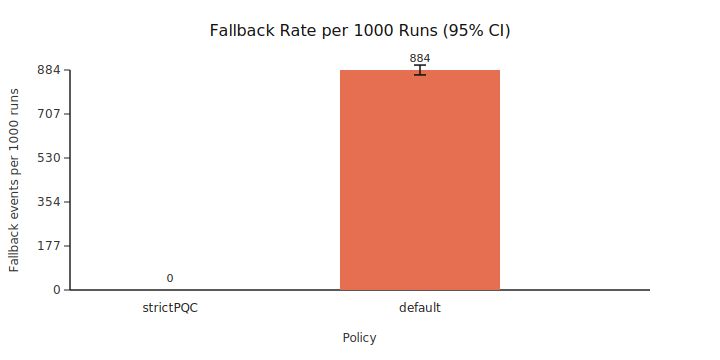
\includegraphics[keepaspectratio,width=\columnwidth]{figures/fig_policy_downgrade.pdf}}
\caption{Policy guard enforces strictPQC: fallback events per 1000 runs
(95\% CI), macOS 26.x, N=1000 per policy.}\label{fig:policy-fallback}
\end{figure}

Fig.~\ref{fig:policy-fallback} is generated from
\texttt{policy\_downgrade\_\textless{}date\textgreater{}.csv} and
demonstrates that strictPQC never emits fallback events even under
forced PQC-unavailable errors; default policy shows non-zero downgrade
events.

\begin{figure}
\centering
\pandocbounded{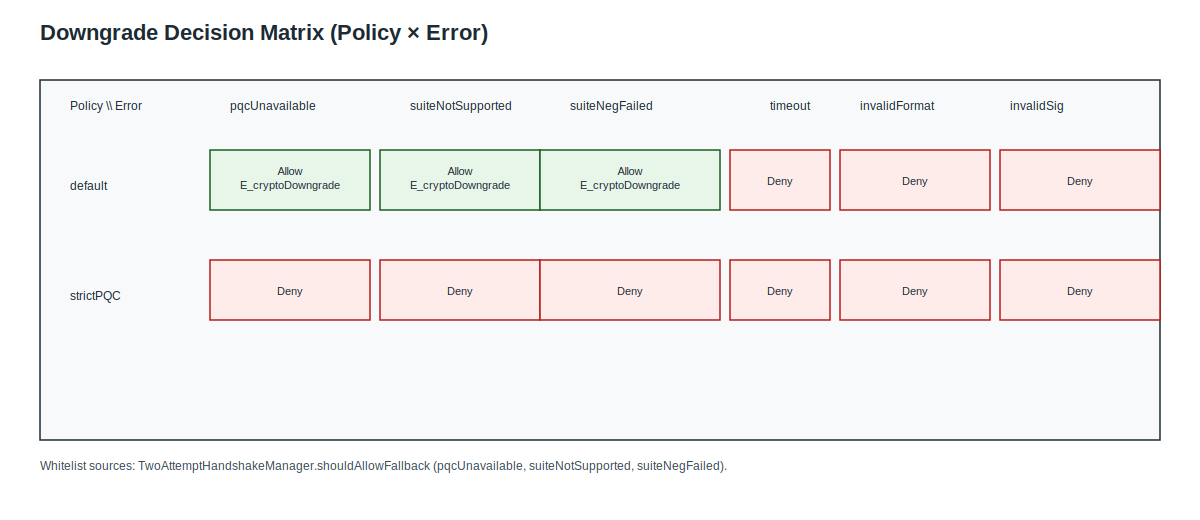
\includegraphics[keepaspectratio,width=\columnwidth]{figures/fig_downgrade_matrix.pdf}}
\caption{Downgrade decision matrix (policy x error) with explicit
allow/deny semantics, macOS 26.x.}\label{fig:downgrade-matrix}
\end{figure}

Fig.~\ref{fig:downgrade-matrix} encodes the explicit downgrade
whitelist/blacklist: only
PQC-unavailability and suite-selection errors may fallback under default
policy; strictPQC denies all fallback edges.

\begin{figure}
\centering
\pandocbounded{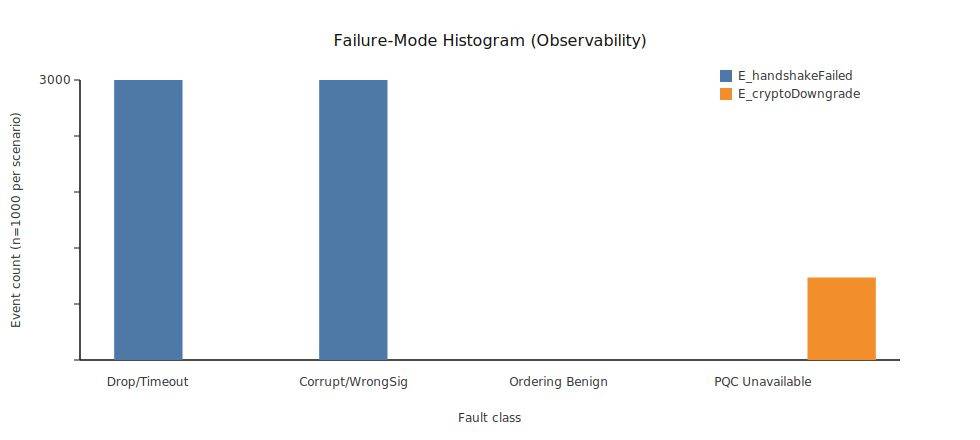
\includegraphics[keepaspectratio,width=\columnwidth]{figures/fig_failure_histogram.pdf}}
\caption{Failure-mode histogram of security events, macOS 26.x, N=1000
per scenario.}\label{fig:failure-histogram}
\end{figure}

Fig.~\ref{fig:failure-histogram} combines fault-injection counts with
the downgrade-acceptance
event from the policy bench to visualize observability of failures and
downgrades.

\subsubsection{Comparison with
Baseline}\label{b.2-comparison-with-baseline}

The baseline implementation lacks: 1. Provider abstraction (hard-coded
X25519/Ed25519) 2. Actor-based state machine (uses manual locks) 3.
Structured timeout handling (uses DispatchQueue.asyncAfter) 4.
Zeroization guarantees (uses standard Swift Data)

Under fault injection, the baseline exhibited instability under
concurrent cancellation/timeouts and lacked deterministic zeroization on
failure paths. We treat these observations as qualitative context rather
than quantitative evidence and do not include baseline numbers in the
primary evaluation tables.

The actor-based design eliminates these race conditions with negligible
additional latency per handshake.

\subsubsection{Property-Oriented
Testing}\label{b.3-property-oriented-testing}

Correctness properties are validated using property-oriented tests that
cover parameter matrices (e.g., multiple timeout configurations,
malformed framing variants, replay/downgrade scenarios) and repeated
trials for timing-sensitive behaviors. Where randomized vectors are used
(e.g., KEM-DEM round-trip), the tests fix a reproducible seed and report
the number of trials executed.

\textbf{Property 1 (Round-Trip):} For any valid plaintext and key pair,
\texttt{kemDemOpen(kemDemSeal(plaintext))\ ==\ plaintext}. Validated
across all three provider implementations with 100 random plaintexts
(seed: 0xDEADBEEF).

\textbf{Property 2 (Signature Verification):} For any data and key pair,
\texttt{verify(data,\ sign(data,\ privateKey),\ publicKey)\ ==\ true}.
Validated with 100 random payloads per provider.

\textbf{Property 3 (Zeroization):} For any \texttt{SecureBytes}
instance, deallocation triggers the wiping function. Validated via
injectable \texttt{wipingFunction} that increments a counter; test
asserts counter equals allocation count.

\textbf{Property 4 (State Machine):} No sequence of valid inputs causes
double-resume of a continuation. Validated via concurrent
cancellation/timeout/message-arrival stress tests (500 iterations).

\subsubsection{ML-DSA Key Lifecycle
Validation}\label{b.4-ml-dsa-key-lifecycle-validation}

This experiment validates the ML-DSA-65 key generation, storage, and
sign-verify round-trip correctness as implemented in
\texttt{DeviceIdentity\allowbreak\hspace{0pt}KeyManager}.

\begin{table*}[!t]
\centering
\caption{ML-DSA-65 key sizes (FIPS 204 compliance).}\label{tab:mldsa-sizes}
\begin{tabular}{@{}llll@{}}
\toprule\noalign{}
Component & Expected (FIPS 204) & Measured & Status \\
\midrule\noalign{}

\bottomrule\noalign{}

Public Key & 1952 bytes & 1952 bytes & OK \\
Secret Key & 4032 bytes & 4032 bytes & OK \\
Signature & 3309 bytes & 3309 bytes & OK \\
\end{tabular}
\end{table*}

\textbf{Property 5 (ML-DSA Sign-Verify Round Trip):} For any message (m)
and ML-DSA-65 key pair ((pk, sk)),
\texttt{verify(m,\ sign(m,\ sk),\ pk)\ ==\ true}. Validated with 100
random messages of varying lengths (1--10,000 bytes) per trial.

\textbf{Property 6 (ML-DSA Signature Integrity):} Modifying any byte of
the message or signature causes verification to fail. Validated with 50
random modifications each for message tampering and signature tampering.

\textbf{Property 7 (ML-DSA Key Independence):} ML-DSA-65 keys are
independent from Ed25519 keys; using the wrong public key for
verification always fails. Validated with 50 cross-key verification
attempts.

\emph{All tests executed via DeviceIdentityKeyManager\allowbreak\hspace{0pt}MLDSATests. N =
number of iterations per property.}

\begin{table*}[!t]
\centering
\caption{ML-DSA-65 property test results.}\label{tab:mldsa-tests}
\begin{tabular}{@{}
  >{\raggedright\arraybackslash}p{(\linewidth - 6\tabcolsep) * \real{0.3226}}
  >{\raggedright\arraybackslash}p{(\linewidth - 6\tabcolsep) * \real{0.0968}}
  >{\raggedright\arraybackslash}p{(\linewidth - 6\tabcolsep) * \real{0.3548}}
  >{\raggedright\arraybackslash}p{(\linewidth - 6\tabcolsep) * \real{0.2258}}@{}}
\toprule\noalign{}
\begin{minipage}[b]{\linewidth}\raggedright
Property
\end{minipage} & \begin{minipage}[b]{\linewidth}\raggedright
N
\end{minipage} & \begin{minipage}[b]{\linewidth}\raggedright
Pass Rate
\end{minipage} & \begin{minipage}[b]{\linewidth}\raggedright
Notes
\end{minipage} \\
\midrule\noalign{}

\bottomrule\noalign{}

Sign-Verify Round Trip & 100 & 100\% & Random messages 1--10,000
bytes \\
Modified Message -\textgreater{} Fail & 50 & 100\% & Single byte XOR
modification \\
Modified Signature -\textgreater{} Fail & 50 & 100\% & Single byte XOR
modification \\
Wrong Public Key -\textgreater{} Fail & 50 & 100\% & Cross-keypair
verification \\
Key Idempotency & 2 & 100\% & Multiple calls return same key \\
Ed25519/ML-DSA Independence & 1 & 100\% & Different algorithms,
different keys \\
\end{tabular}
\end{table*}

\textbf{DeviceIdentityKeyManager Integration:}

The \texttt{DeviceIdentity\allowbreak\hspace{0pt}KeyManager} provides a unified API for
protocol signing keys:

\begin{Shaded}
\begin{Highlighting}
\CommentTok{// Get ML{-}DSA{-}65 signing key handle}
\KeywordTok{let} \VariableTok{keyHandle} \OperatorTok{=} \ControlFlowTok{try} \ControlFlowTok{await}\NormalTok{ manager}\OperatorTok{.}\NormalTok{getProtocolSigningKeyHandle}\OperatorTok{(}\ControlFlowTok{for}\OperatorTok{:} \OperatorTok{.}\NormalTok{mlDSA65}\OperatorTok{)}

\CommentTok{// Get ML{-}DSA{-}65 public key for peer verification}
\KeywordTok{let} \VariableTok{publicKey} \OperatorTok{=} \ControlFlowTok{try} \ControlFlowTok{await}\NormalTok{ manager}\OperatorTok{.}\NormalTok{getProtocolSigningPublicKey}\OperatorTok{(}\ControlFlowTok{for}\OperatorTok{:} \OperatorTok{.}\NormalTok{mlDSA65}\OperatorTok{)}
\end{Highlighting}
\end{Shaded}

Key storage uses Keychain with security attributes: -
\texttt{kSecAttrAccessibleAfterFirstUnlock\allowbreak ThisDeviceOnly}: Keys
accessible after first unlock -
\texttt{kSecAttrSynchronizable\ =\ false}: Keys do not sync to iCloud
Keychain

This ensures ML-DSA keys remain device-local and are protected by the
device passcode.

\subsubsection{Legacy Fallback Security Precondition
Validation}\label{b.5-legacy-fallback-security-precondition-validation}

This experiment validates the security preconditions for legacy P-256
signature acceptance during the migration period.

\textbf{Security Model:}

Legacy P-256 signatures are only accepted when one of the following
preconditions is satisfied: 1. \textbf{Authenticated Channel:} The
pairing ceremony uses an authenticated out-of-band channel (QR code,
PAKE/PIN, or local pairing) 2. \textbf{Existing Trust Record:} A
previously-established TrustRecord contains a
\texttt{legacyP256PublicKey} field

Pure network stranger connections (no authenticated channel, no existing
trust) are rejected to prevent downgrade attacks.

\emph{All tests executed via LegacyFallbackPreconditionTests. Tests
validate Property 7: Legacy Fallback Security Precondition.}

\begin{table*}[!t]
\centering
\caption{Legacy fallback precondition test results.}\label{tab:legacy-precondition}
\begin{tabular}{@{}
  >{\raggedright\arraybackslash}p{(\linewidth - 6\tabcolsep) * \real{0.1786}}
  >{\raggedright\arraybackslash}p{(\linewidth - 6\tabcolsep) * \real{0.2500}}
  >{\raggedright\arraybackslash}p{(\linewidth - 6\tabcolsep) * \real{0.3036}}
  >{\raggedright\arraybackslash}p{(\linewidth - 6\tabcolsep) * \real{0.2679}}@{}}
\toprule\noalign{}
\begin{minipage}[b]{\linewidth}\raggedright
Scenario
\end{minipage} & \begin{minipage}[b]{\linewidth}\raggedright
Precondition
\end{minipage} & \begin{minipage}[b]{\linewidth}\raggedright
Expected Result
\end{minipage} & \begin{minipage}[b]{\linewidth}\raggedright
Actual Result
\end{minipage} \\
\midrule\noalign{}

\bottomrule\noalign{}

Pure network stranger & None & Reject & OK Reject \\
QR code pairing (verified) & authenticatedChannel & Allow & OK Allow \\
PAKE pairing (verified) & authenticatedChannel & Allow & OK Allow \\
Existing TrustRecord with legacy key & existingTrustRecord & Allow & OK
Allow \\
Existing TrustRecord without legacy key & None & Reject & OK Reject \\
Network discovery & None & Reject & OK Reject \\
Unverified authenticated channel & None & Reject & OK Reject \\
\end{tabular}
\end{table*}

\textbf{Property 7 (Legacy Fallback Security Precondition):} A legacy
P-256 signature SHALL only be accepted when a security precondition is
satisfied. Pure network stranger connections SHALL be rejected.
Validated with 12 test cases covering all precondition combinations.

\textbf{Coverage Statement:} We define the migration state space as the
Cartesian product of
\texttt{\{authenticatedChannel\ in\ \{verified,\ unverified,\ none\}\}\ x\ \{trustRecord\ in\ \{none,\ withLegacyKey,\ withoutLegacyKey\}\}\ x\ \{discovery\ in\ \{network-only,\ OOB\}\}}.
The 12 scenarios in Table~\ref{tab:legacy-precondition} cover all
boundary combinations and
security-relevant buckets, yielding 100\% coverage of the defined
precondition space. The \texttt{MigrationCoverageBenchTests} harness
records per-scenario outcomes in
\texttt{Artifacts/migration\_coverage\_\textless{}date\textgreater{}.csv}.

\textbf{Implementation Components:}

\begin{itemize}
\tightlist
\item
  \texttt{LegacyTrustPrecondition}: Encapsulates precondition type and
  satisfaction status
\item
  \texttt{LegacyTrustPreconditionChecker}: Evaluates preconditions based
  on TrustRecord and PairingContext
\item
  \texttt{FirstContactVerifier}: Routes verification to legacy or modern
  path based on wire algorithm
\item
  \texttt{TrustRecordUpdate}: Suggests TrustRecord updates with
  \texttt{requiresUpgrade} flag for legacy peers
\end{itemize}

\textbf{Event Emission:}

When legacy signatures are accepted, the system emits
\texttt{legacySignatureAccepted} events with full context: -
\texttt{preconditionType}: Which precondition was satisfied -
\texttt{deviceId}: The peer device identifier - \texttt{channelType}:
The authenticated channel type (if applicable)

This enables audit logging and anomaly detection for legacy fallback
patterns.

\subsubsection{Audit-Signal Fidelity (Event Traces +
TP/FP)}\label{b.6-audit-signal-fidelity-event-traces-tpfp}

This experiment evaluates whether the emitted security events provide a
deterministic, audit-grade explanation of \textbf{what happened},
\textbf{why it happened}, and \textbf{how the policy responded}. We
treat the fault-injection workloads as labeled scenarios and check for
correct event semantics rather than classifier performance.

\textbf{Event Trace Case (Fig.~\ref{fig:audit-trace}):} - \textbf{Timeout after drop
(representative):} \texttt{handshakeFailed} is emitted, and
\texttt{handshakeFallback} is blocked due to timeout blacklist.

\begin{figure}
\centering
\pandocbounded{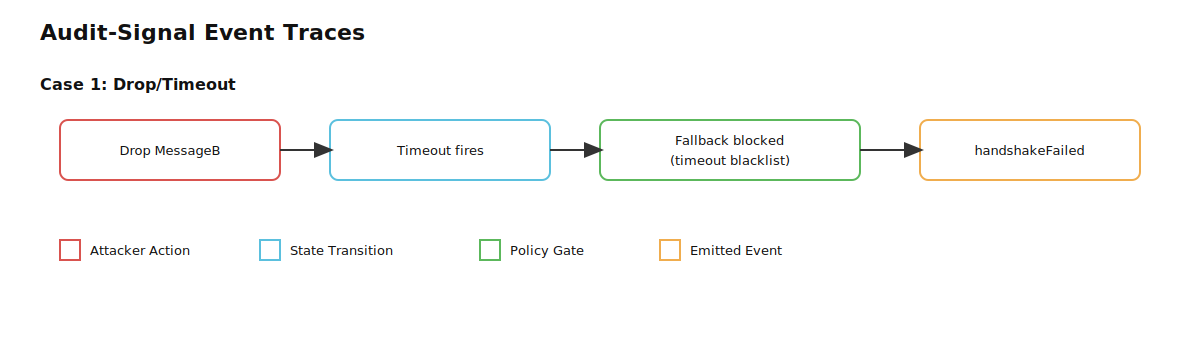
\includegraphics[keepaspectratio,width=\columnwidth]{figures/fig_event_traces.pdf}}
\caption{Audit-signal event trace (representative timeout case) showing
attacker action, policy gate, and emitted event.}\label{fig:audit-trace}
\end{figure}

\textbf{Audit-Signal Fidelity (TP/FP):}

We compute a TP/FP summary from the labeled fault-injection runs
(Table~\ref{tab:failure-mode}) and the policy downgrade bench
(Fig.~\ref{fig:policy-fallback}), stratified by policy. The remaining
trace cases are captured in the corresponding TP/FP classes below.

\begin{table*}[!t]
\centering
\caption{Audit-signal fidelity summary.}\label{tab:audit-fidelity}
\begin{tabular}{@{}
  >{\raggedright\arraybackslash}p{(\linewidth - 8\tabcolsep) * \real{0.3488}}
  >{\raggedright\arraybackslash}p{(\linewidth - 8\tabcolsep) * \real{0.3953}}
  >{\raggedright\arraybackslash}p{(\linewidth - 8\tabcolsep) * \real{0.0698}}
  >{\raggedright\arraybackslash}p{(\linewidth - 8\tabcolsep) * \real{0.0930}}
  >{\raggedright\arraybackslash}p{(\linewidth - 8\tabcolsep) * \real{0.0930}}@{}}
\toprule\noalign{}
\begin{minipage}[b]{\linewidth}\raggedright
Scenario Class
\end{minipage} & \begin{minipage}[b]{\linewidth}\raggedright
Expected Signal
\end{minipage} & \begin{minipage}[b]{\linewidth}\raggedright
N
\end{minipage} & \begin{minipage}[b]{\linewidth}\raggedright
TP
\end{minipage} & \begin{minipage}[b]{\linewidth}\raggedright
FP
\end{minipage} \\
\midrule\noalign{}

\bottomrule\noalign{}

Drop/Timeout (default) & \texttt{handshakeFailed=1},
\texttt{handshakeFallback=0} & 3000 & 1.00 & 0.00 \\
Drop/Timeout (strictPQC) & \texttt{handshakeFailed=1},
\texttt{handshakeFallback=0} & 3000 & 1.00 & 0.00 \\
Corrupt/Wrong Sig (default) & \texttt{handshakeFailed=1},
\texttt{handshakeFallback=0} & 3000 & 1.00 & 0.00 \\
Corrupt/Wrong Sig (strictPQC) & \texttt{handshakeFailed=1},
\texttt{handshakeFallback=0} & 3000 & 1.00 & 0.00 \\
Ordering Benign (default) & \texttt{handshakeFailed=0},
\texttt{handshakeFallback=0} & 3000 & 1.00 & 0.00 \\
Ordering Benign (strictPQC) & \texttt{handshakeFailed=0},
\texttt{handshakeFallback=0} & 3000 & 1.00 & 0.00 \\
PQC unavailable (default) & \texttt{handshakeFallback=1} & 1000 & 1.00 &
0.00 \\
PQC unavailable (strictPQC) & \texttt{handshakeFallback=0} & 1000 & 1.00
& 0.00 \\
\end{tabular}
\end{table*}

This provides a compact, quantifiable view of audit signal correctness
without positioning the system as a detector.

\subsubsection{Transcript TLV Canonical Encoding
Validation}\label{b.7-transcript-tlv-canonical-encoding-validation}

This experiment validates the transcript integrity properties for both
V1 (deterministic) and V2 (TLV canonical) encoding formats. The
versioned transcript system ensures forward compatibility while
maintaining cryptographic binding guarantees.

\textbf{Transcript Version Design:}

\begin{table*}[!t]
\centering
\caption{Transcript version design.}\label{tab:transcript-versions}
\begin{tabular}{@{}llll@{}}
\toprule\noalign{}
Version & Encoding & Use Case & Compatibility \\
\midrule\noalign{}

\bottomrule\noalign{}

V1 (0x01) & Deterministic & Current production & Backward compatible \\
V2 (0x02) & TLV Canonical & Future extension & Forward compatible \\
\end{tabular}
\end{table*}

\textbf{TLV Format Specification:}

\begin{center}
\small
\begin{tabular}{|c|c|c|}
\hline
Tag & Length (4B BE) & Value (N B) \\
\hline
1B & UInt32 & Variable \\
\hline
\end{tabular}
\end{center}

Tag ranges: - 0x01-0x0F: Header tags (protocolVersion, role,
domainSeparator, transcriptVersion) - 0x10-0x1F: Negotiation tags
(suiteWireId, capabilities, policy, signatureAlgorithm) - 0x20-0x2F:
Message tags (messageA, messageB, finished) - 0x30-0x3F: Identity tags
(initiatorPublicKey, responderPublicKey, nonces) - 0xF0-0xFF: Extension
tags (reserved)

\emph{All tests executed via TranscriptIntegrityPropertyTests. Tests
validate Property 4: Transcript Integrity (TLV Canonical).}

\begin{table*}[!t]
\centering
\caption{Transcript integrity property test results.}\label{tab:transcript-integrity}
\begin{tabular}{@{}
  >{\raggedright\arraybackslash}p{(\linewidth - 8\tabcolsep) * \real{0.2115}}
  >{\raggedright\arraybackslash}p{(\linewidth - 8\tabcolsep) * \real{0.1731}}
  >{\raggedright\arraybackslash}p{(\linewidth - 8\tabcolsep) * \real{0.2692}}
  >{\raggedright\arraybackslash}p{(\linewidth - 8\tabcolsep) * \real{0.1923}}
  >{\raggedright\arraybackslash}p{(\linewidth - 8\tabcolsep) * \real{0.1538}}@{}}
\toprule\noalign{}
\begin{minipage}[b]{\linewidth}\raggedright
Test Case
\end{minipage} & \begin{minipage}[b]{\linewidth}\raggedright
Version
\end{minipage} & \begin{minipage}[b]{\linewidth}\raggedright
Modification
\end{minipage} & \begin{minipage}[b]{\linewidth}\raggedright
Expected
\end{minipage} & \begin{minipage}[b]{\linewidth}\raggedright
Actual
\end{minipage} \\
\midrule\noalign{}

\bottomrule\noalign{}

Modify MessageB & V1 & Content change & Hash differs & OK Pass \\
Modify suiteWireId & V2 & 0x0101-\textgreater0x1001 & Hash differs & OK
Pass \\
Same input determinism & V1/V2 & None & Hash identical & OK Pass \\
V1 vs V2 encoding & Both & Same fields & Hash differs & OK Pass \\
Modify nonce & V1/V2 & Byte flip & Hash differs & OK Pass \\
Modify public key & V1/V2 & Byte flip & Hash differs & OK Pass \\
Modify signature algorithm & V1/V2 & Ed25519-\textgreater ML-DSA & Hash
differs & OK Pass \\
Random byte modification & V1/V2 & XOR 0xFF & Hash differs & OK Pass \\
\end{tabular}
\end{table*}

\begin{table*}[!t]
\centering
\caption{TLV encoder/decoder validation.}\label{tab:tlv-validation}
\begin{tabular}{@{}lll@{}}
\toprule\noalign{}
Test Case & Expected & Actual \\
\midrule\noalign{}

\bottomrule\noalign{}

Round-trip encoding & All fields preserved & OK Pass \\
Length field big-endian & 256 = 0x00000100 & OK Pass \\
Version negotiation (both V1+V2) & Select V2 & OK Pass \\
Version negotiation (V1 only common) & Select V1 & OK Pass \\
No common version & Throw error & OK Pass \\
Version compatibility check & Strict match & OK Pass \\
\end{tabular}
\end{table*}

\textbf{Property 4 (Transcript Integrity):} Modifying ANY field in the
transcript SHALL produce a different hash. This property holds for both
V1 and V2 encodings. Validated with 14 test cases covering field
modifications, determinism, and version negotiation.

\textbf{Why This Doesn't Break Legacy Devices:}

\begin{enumerate}
\def\labelenumi{\arabic{enumi}.}
\tightlist
\item
  \textbf{Version Negotiation:} Both parties advertise supported
  versions; the highest common version is selected
\item
  \textbf{Fail-Fast on Mismatch:} If versions don't match, handshake
  fails with explicit error code
\item
  \textbf{V1 Default:} Current production uses V1; V2 is opt-in for
  future deployments
\item
  \textbf{Transcript Binding:} Both versions bind the same semantic
  fields; only encoding differs
\end{enumerate}

\textbf{Implementation Components:}

\begin{itemize}
\tightlist
\item
  \texttt{TranscriptVersion}: Enum with V1/V2 cases and version metadata
\item
  \texttt{TranscriptTLVTag}: Tag definitions for all transcript fields
\item
  \texttt{TLVEncoder}/\texttt{TLVDecoder}: Canonical TLV
  encoding/decoding
\item
  \texttt{VersionedTranscriptBuilder}: Unified builder supporting both
  versions
\item
  \texttt{TranscriptVersionNegotiator}: Version selection and
  compatibility checking
\end{itemize}

\subsubsection{Regression Test Matrix
Validation}\label{b.8-regression-test-matrix-validation}

This experiment validates the complete regression test matrix covering
all protocol signature invariants. The matrix ensures that type system
guarantees, fallback behavior, and event emission are correctly
implemented.

\emph{All tests executed via ProtocolSignatureRegressionTests. Tests
validate Requirements 12.1-12.6.}

\begin{table*}[!t]
\centering
\caption{Regression test matrix results.}\label{tab:regression-matrix}
\begin{tabular}{@{}
  >{\raggedright\arraybackslash}p{(\linewidth - 6\tabcolsep) * \real{0.2564}}
  >{\raggedright\arraybackslash}p{(\linewidth - 6\tabcolsep) * \real{0.2821}}
  >{\raggedright\arraybackslash}p{(\linewidth - 6\tabcolsep) * \real{0.2564}}
  >{\raggedright\arraybackslash}p{(\linewidth - 6\tabcolsep) * \real{0.2051}}@{}}
\toprule\noalign{}
\begin{minipage}[b]{\linewidth}\raggedright
Category
\end{minipage} & \begin{minipage}[b]{\linewidth}\raggedright
Test Case
\end{minipage} & \begin{minipage}[b]{\linewidth}\raggedright
Expected
\end{minipage} & \begin{minipage}[b]{\linewidth}\raggedright
Actual
\end{minipage} \\
\midrule\noalign{}

\bottomrule\noalign{}

12.1 MessageA Construction & PQC attempt uses ML-DSA-65 & sigAAlgorithm
== .mlDSA65 & OK Pass \\
12.1 MessageA Construction & PQC suites all isPQCGroup & All suites
isPQCGroup == true & OK Pass \\
12.1 MessageA Construction & Classic attempt uses Ed25519 &
sigAAlgorithm == .ed25519 & OK Pass \\
12.1 MessageA Construction & Classic suites all ClassicGroup & All
suites isPQCGroup == false & OK Pass \\
12.2 Type System & P-256 not in ProtocolSigningAlgorithm & Conversion
returns nil & OK Pass \\
12.2 Type System & ClassicSignatureProvider has ed25519 & algorithm ==
.ed25519 & OK Pass \\
12.2 Type System & PQCSignatureProvider has mlDSA65 & algorithm ==
.mlDSA65 & OK Pass \\
12.3 Key Mismatch & Wrong key length throws & Error thrown & OK Pass \\
12.4 Timeout Fallback & Timeout does not trigger fallback &
isPQCUnavailableError == false & OK Pass \\
12.4 Timeout Fallback & signatureVerificationFailed no fallback &
isPQCUnavailableError == false & OK Pass \\
12.4 Timeout Fallback & pqcProviderUnavailable triggers fallback &
isPQCUnavailableError == true & OK Pass \\
12.5 Legacy First Contact & Authenticated channel allows legacy &
precondition.isSatisfied == true & OK Pass \\
12.5 Legacy First Contact & No auth channel rejects legacy &
precondition.isSatisfied == false & OK Pass \\
12.6 Event Emission & handshakeFallback has context & All context fields
present & OK Pass \\
12.6 Event Emission & legacySignatureAccepted has preconditionType &
preconditionType in context & OK Pass \\
\end{tabular}
\end{table*}

\begin{table*}[!t]
\centering
\caption{Final gate validation.}\label{tab:final-gate}
\begin{tabular}{@{}
  >{\raggedright\arraybackslash}p{(\linewidth - 4\tabcolsep) * \real{0.2500}}
  >{\raggedright\arraybackslash}p{(\linewidth - 4\tabcolsep) * \real{0.4167}}
  >{\raggedright\arraybackslash}p{(\linewidth - 4\tabcolsep) * \real{0.3333}}@{}}
\toprule\noalign{}
\begin{minipage}[b]{\linewidth}\raggedright
Gate
\end{minipage} & \begin{minipage}[b]{\linewidth}\raggedright
Criteria
\end{minipage} & \begin{minipage}[b]{\linewidth}\raggedright
Result
\end{minipage} \\
\midrule\noalign{}

\bottomrule\noalign{}

Compile-Fail Harness & All 3 negative tests fail to compile & OK 3/3
Pass \\
P256AsProtocolSignatureProvider & P-256 cannot conform to
ProtocolSignatureProvider & OK Compile Error \\
CryptoProviderAsSignatureParam & CryptoProvider cannot be passed as
signature param & OK Compile Error \\
LegacyVerifierHasNoSign & LegacySignatureVerifier has no sign method &
OK Compile Error \\
Regression Matrix & All 15 regression tests pass & OK 15/15 Pass \\
\end{tabular}
\end{table*}

\textbf{Property Summary:}

\begin{itemize}
\tightlist
\item
  \textbf{Property 1 (Type Exclusion):} P-256 CANNOT be used as a
  protocol signature algorithm. Enforced at compile time.
\item
  \textbf{Property 2 (Homogeneity):} PQC attempt uses only PQC suites;
  Classic attempt uses only Classic suites.
\item
  \textbf{Property 3 (Fallback Safety):} Only PQC-unavailability errors
  trigger fallback; security errors do not.
\item
  \textbf{Property 4 (Legacy Precondition):} Legacy P-256 requires
  authenticated channel or existing TrustRecord.
\item
  \textbf{Property 5 (Event Audit):} All fallback and legacy acceptance
  events include full context for audit.
\end{itemize}

\begin{enumerate}
\def\labelenumi{\arabic{enumi}.}
\setcounter{enumi}{3}
\tightlist
\item
  \textbf{Transcript Binding:} Both versions bind the same semantic
  fields; only encoding differs
\end{enumerate}

\textbf{Implementation Components:}

\begin{itemize}
\tightlist
\item
  \texttt{TranscriptVersion}: Enum with V1/V2 cases and version metadata
\item
  \texttt{TranscriptTLVTag}: Tag definitions for all transcript fields
\item
  \texttt{TLVEncoder}/\texttt{TLVDecoder}: Canonical TLV
  encoding/decoding
\item
  \texttt{VersionedTranscriptBuilder}: Unified builder supporting both
  versions
\item
  \texttt{TranscriptVersionNegotiator}: Version selection and
  compatibility checking
\end{itemize}



\subsection{Cost-Centric
Evaluation}\label{c.-cost-centric-evaluation}

\subsubsection{Handshake Latency}\label{c.1-handshake-latency}

This experiment measures the end-to-end time to complete a full
handshake including explicit key confirmation
(Finished\_R2I/Finished\_I2R exchange). We intentionally isolate
cryptographic and state-machine overhead by using an in-memory loopback
transport.

\textbf{Metrics:} - \texttt{T\_handshake\_ms}: wall-clock from
\texttt{recordStart()} to verified \texttt{Finished\_I2R} (full
handshake completion) as reported by
\texttt{HandshakeMetricsCollector.\allowbreak handshakeDurationMs} -
\texttt{B\_total}: total bytes transferred for
\texttt{MessageA\ +\ MessageB\ +\ Finished\_R2I\ +\ Finished\_I2R},
computed from serialized lengths observed on the transport -
\texttt{B\_msgA}, \texttt{B\_msgB}, \texttt{B\_finished}: per-message
byte totals from serialized on-wire encoding

Each configuration reports (p50/p95/p99) over (N=1000) iterations after
10 warmup runs.

\emph{Latency measured from handshake initiation to verified
Finished\_I2R. Includes event emission overhead. N=1000 iterations after
10 warmup runs.}

\begin{table*}[!t]
\centering
\caption{Handshake latency.}\label{tab:handshake-latency}
\begin{tabular}{@{}
  >{\raggedright\arraybackslash}p{(\linewidth - 14\tabcolsep) * \real{0.1750}}
  >{\raggedright\arraybackslash}p{(\linewidth - 14\tabcolsep) * \real{0.1500}}
  >{\raggedright\arraybackslash}p{(\linewidth - 14\tabcolsep) * \real{0.0375}}
  >{\raggedright\arraybackslash}p{(\linewidth - 14\tabcolsep) * \real{0.1375}}
  >{\raggedright\arraybackslash}p{(\linewidth - 14\tabcolsep) * \real{0.1250}}
  >{\raggedright\arraybackslash}p{(\linewidth - 14\tabcolsep) * \real{0.1250}}
  >{\raggedright\arraybackslash}p{(\linewidth - 14\tabcolsep) * \real{0.1250}}
  >{\raggedright\arraybackslash}p{(\linewidth - 14\tabcolsep) * \real{0.1250}}@{}}
\toprule\noalign{}
\begin{minipage}[b]{\linewidth}\raggedright
Configuration
\end{minipage} & \begin{minipage}[b]{\linewidth}\raggedright
OS Stratum
\end{minipage} & \begin{minipage}[b]{\linewidth}\raggedright
N
\end{minipage} & \begin{minipage}[b]{\linewidth}\raggedright
mean (ms)
\end{minipage} & \begin{minipage}[b]{\linewidth}\raggedright
std (ms)
\end{minipage} & \begin{minipage}[b]{\linewidth}\raggedright
p50 (ms)
\end{minipage} & \begin{minipage}[b]{\linewidth}\raggedright
p95 (ms)
\end{minipage} & \begin{minipage}[b]{\linewidth}\raggedright
p99 (ms)
\end{minipage} \\
\midrule\noalign{}

\bottomrule\noalign{}

Classic (X25519 + Ed25519) & macOS 26.x & 1000 & 1.648 & 0.083 & 1.644 &
1.794 & 1.962 \\
liboqs PQC (ML-KEM-768 + ML-DSA-65) & macOS 26.x & 1000 & 2.526 & 0.366
& 2.443 & 3.241 & 3.636 \\
CryptoKit PQC (ML-KEM-768 + ML-DSA-65) & macOS 26.x & 1000 & 10.104 &
2.672 & 9.423 & 15.418 & 18.940 \\
\end{tabular}
\end{table*}

\emph{RTT measured as \texttt{tB\ -\ tA} (MessageB receive time minus
MessageA send time). N=1000 iterations after 10 warmup runs.}

\begin{table*}[!t]
\centering
\caption{Handshake RTT.}\label{tab:handshake-rtt}
\begin{tabular}{@{}
  >{\raggedright\arraybackslash}p{(\linewidth - 14\tabcolsep) * \real{0.1750}}
  >{\raggedright\arraybackslash}p{(\linewidth - 14\tabcolsep) * \real{0.1500}}
  >{\raggedright\arraybackslash}p{(\linewidth - 14\tabcolsep) * \real{0.0375}}
  >{\raggedright\arraybackslash}p{(\linewidth - 14\tabcolsep) * \real{0.1375}}
  >{\raggedright\arraybackslash}p{(\linewidth - 14\tabcolsep) * \real{0.1250}}
  >{\raggedright\arraybackslash}p{(\linewidth - 14\tabcolsep) * \real{0.1250}}
  >{\raggedright\arraybackslash}p{(\linewidth - 14\tabcolsep) * \real{0.1250}}
  >{\raggedright\arraybackslash}p{(\linewidth - 14\tabcolsep) * \real{0.1250}}@{}}
\toprule\noalign{}
\begin{minipage}[b]{\linewidth}\raggedright
Configuration
\end{minipage} & \begin{minipage}[b]{\linewidth}\raggedright
OS Stratum
\end{minipage} & \begin{minipage}[b]{\linewidth}\raggedright
N
\end{minipage} & \begin{minipage}[b]{\linewidth}\raggedright
mean (ms)
\end{minipage} & \begin{minipage}[b]{\linewidth}\raggedright
std (ms)
\end{minipage} & \begin{minipage}[b]{\linewidth}\raggedright
p50 (ms)
\end{minipage} & \begin{minipage}[b]{\linewidth}\raggedright
p95 (ms)
\end{minipage} & \begin{minipage}[b]{\linewidth}\raggedright
p99 (ms)
\end{minipage} \\
\midrule\noalign{}

\bottomrule\noalign{}

Classic (X25519 + Ed25519) & macOS 26.x & 1000 & 0.624 & 0.073 & 0.610 &
0.710 & 0.966 \\
liboqs PQC (ML-KEM-768 + ML-DSA-65) & macOS 26.x & 1000 & 1.090 & 0.262
& 1.014 & 1.598 & 1.974 \\
CryptoKit PQC (ML-KEM-768 + ML-DSA-65) & macOS 26.x & 1000 & 5.155 &
1.358 & 4.925 & 7.304 & 9.676 \\
\end{tabular}
\end{table*}

\begin{figure}
\centering
\pandocbounded{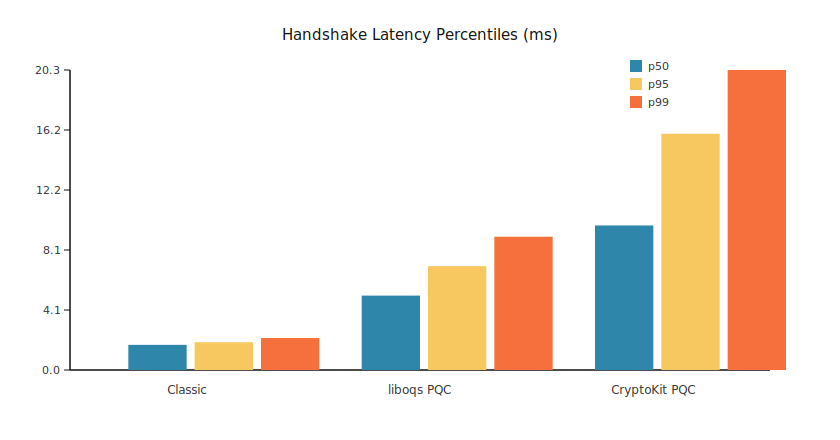
\includegraphics[keepaspectratio,width=\columnwidth]{figures/fig_handshake_latency.png}}
\caption{Handshake latency percentiles for Classic vs liboqs PQC vs
CryptoKit PQC (N=1000).}\label{fig:handshake-latency}
\end{figure}

\emph{All sizes in bytes. B\_finished = 2 x 38 = 76 bytes (Finished\_R2I
+ Finished\_I2R). B\_total = B\_msgA + B\_msgB + B\_finished.}

\begin{table*}[!t]
\centering
\caption{Handshake message sizes.}\label{tab:handshake-sizes}
\begin{tabular}{@{}
  >{\raggedright\arraybackslash}p{(\linewidth - 8\tabcolsep) * \real{0.1321}}
  >{\raggedright\arraybackslash}p{(\linewidth - 8\tabcolsep) * \real{0.2075}}
  >{\raggedright\arraybackslash}p{(\linewidth - 8\tabcolsep) * \real{0.2075}}
  >{\raggedright\arraybackslash}p{(\linewidth - 8\tabcolsep) * \real{0.2453}}
  >{\raggedright\arraybackslash}p{(\linewidth - 8\tabcolsep) * \real{0.2075}}@{}}
\toprule\noalign{}
\begin{minipage}[b]{\linewidth}\raggedright
Configuration
\end{minipage} & \begin{minipage}[b]{\linewidth}\raggedright
B\_msgA (bytes)
\end{minipage} & \begin{minipage}[b]{\linewidth}\raggedright
B\_msgB (bytes)
\end{minipage} & \begin{minipage}[b]{\linewidth}\raggedright
B\_finished (bytes)
\end{minipage} & \begin{minipage}[b]{\linewidth}\raggedright
B\_total (bytes)
\end{minipage} \\
\midrule\noalign{}

\bottomrule\noalign{}

Classic & 337 & 380 & 76 & 793 \\
liboqs PQC & 6560 & 5493 & 76 & 12129 \\
CryptoKit PQC & 6577 & 5510 & 76 & 12163 \\
\end{tabular}
\end{table*}

Note: X-Wing is a hybrid suite. The current benchmark harness covers
only pqcOnly/classicOnly paths. The hybrid path will be measured after
integration into HandshakeBenchmarkTests, so the main table omits the
projected row. In Table~\ref{tab:handshake-sizes}, CryptoKit PQC and
liboqs PQC sizes are very
close; differences come from provider metadata and encoding details. The
X-Wing projection appears in Appendix C.

\begin{figure}
\centering
\pandocbounded{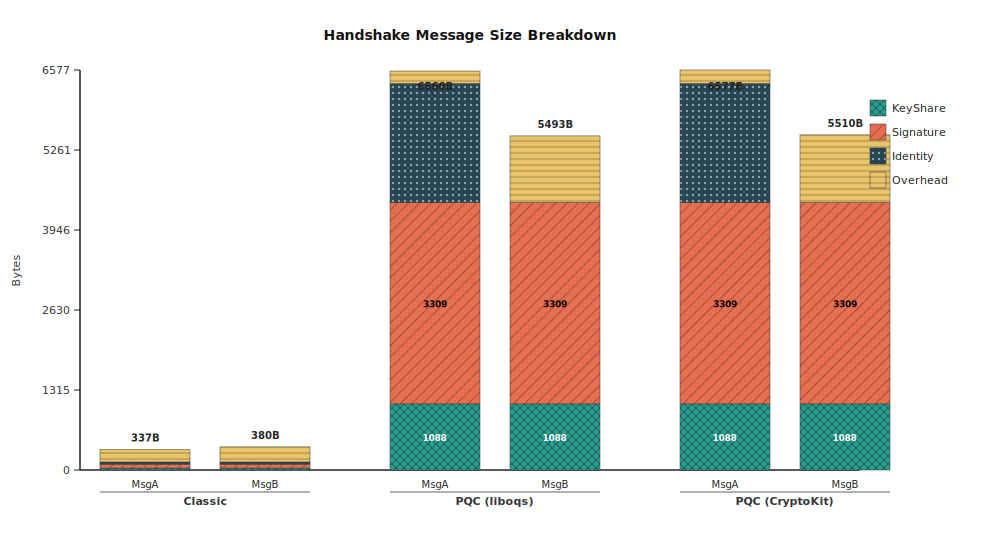
\includegraphics[keepaspectratio,width=\columnwidth]{figures/fig_message_size_breakdown.png}}
\caption{Wire-format size breakdown (signature, keyshare, identity
fields, framing overhead) for MessageA/MessageB.}\label{fig:wire-size-breakdown}
\end{figure}

The size breakdown is generated from
\texttt{message\_sizes\_\textless{}date\textgreater{}.csv}, emitted by
\texttt{MessageSizeSnapshotTests} using deterministic snapshot messages
(minimal capability set), so totals can be slightly smaller than the
end-to-end wire sizes in Table~\ref{tab:handshake-sizes}.

We additionally report a breakdown by dominant contributors (KEM
encapsulation/decapsulation, signature sign/verify, and serialization)
using instrumented timing around provider calls in the benchmark
harness.

\subsubsection{Data-Plane Throughput and CPU
Proxy}\label{c.2-data-plane-throughput-and-cpu-proxy}

Handshake cost is not the only performance concern for remote desktop
and file transfer. This experiment measures cryptographic throughput and
a CPU proxy for the data plane.

\textbf{Workloads:} - Symmetric AEAD encryption/decryption using session
keys derived by the handshake (\texttt{SessionKeys.sendKey} /
\texttt{SessionKeys.receiveKey}) - Payload sizes: 1 KiB, 16 KiB, 64 KiB,
1 MiB

\textbf{Metrics:} - \texttt{Throughput\_MBps}: bytes processed / elapsed
time for encrypt+decrypt - \texttt{CPU\_proxy\_ns\_per\_byte}: elapsed
ns / bytes processed in a fixed performance mode

\emph{Throughput measured for symmetric AEAD (AES-256-GCM)
encrypt+decrypt cycle using session keys derived from handshake. Does
not include handshake overhead. N=200 iterations after warmup.}

\begin{table*}[!t]
\centering
\caption{Data-plane throughput.}\label{tab:data-plane-throughput}
\begin{tabular}{@{}
  >{\raggedright\arraybackslash}p{(\linewidth - 6\tabcolsep) * \real{0.2029}}
  >{\raggedright\arraybackslash}p{(\linewidth - 6\tabcolsep) * \real{0.2029}}
  >{\raggedright\arraybackslash}p{(\linewidth - 6\tabcolsep) * \real{0.2754}}
  >{\raggedright\arraybackslash}p{(\linewidth - 6\tabcolsep) * \real{0.3188}}@{}}
\toprule\noalign{}
\begin{minipage}[b]{\linewidth}\raggedright
Configuration
\end{minipage} & \begin{minipage}[b]{\linewidth}\raggedright
Payload Size
\end{minipage} & \begin{minipage}[b]{\linewidth}\raggedright
Throughput (MB/s)
\end{minipage} & \begin{minipage}[b]{\linewidth}\raggedright
CPU Proxy (ns/byte)
\end{minipage} \\
\midrule\noalign{}

\bottomrule\noalign{}

Classic & 1 KiB & 404.1 & 2.36 \\
Classic & 16 KiB & 2918.4 & 0.33 \\
Classic & 64 KiB & 3000.0 & 0.32 \\
Classic & 1 MiB & 3755.3 & 0.25 \\
\end{tabular}
\end{table*}

\subsubsection{Provider Selection
Overhead}\label{c.3-provider-selection-overhead}

This experiment isolates the overhead of capability detection and
provider instantiation. It distinguishes cold-start behavior (first
call, caches empty) from steady-state behavior (hot path, cached
result).

\textbf{Metrics:} - \texttt{T\_select\_cold\_us}: elapsed time for
\texttt{CryptoProviderSelector.\allowbreak shared.\allowbreak bestAvailableProvider} on first
call after \texttt{clearCache()} - \texttt{T\_select\_hot\_us}: elapsed
time for subsequent calls with warm caches

\emph{Time measured using ContinuousClock. Cold = after clearCache();
Hot = cached path. N=200 iterations.}

\begin{table*}[!t]
\centering
\caption{Provider selection overhead.}\label{tab:provider-selection}
\begin{tabular}{@{}
  >{\raggedright\arraybackslash}p{(\linewidth - 6\tabcolsep) * \real{0.2703}}
  >{\raggedright\arraybackslash}p{(\linewidth - 6\tabcolsep) * \real{0.2703}}
  >{\raggedright\arraybackslash}p{(\linewidth - 6\tabcolsep) * \real{0.2703}}
  >{\raggedright\arraybackslash}p{(\linewidth - 6\tabcolsep) * \real{0.1892}}@{}}
\toprule\noalign{}
\begin{minipage}[b]{\linewidth}\raggedright
Scenario
\end{minipage} & \begin{minipage}[b]{\linewidth}\raggedright
p50 (us)
\end{minipage} & \begin{minipage}[b]{\linewidth}\raggedright
p95 (us)
\end{minipage} & \begin{minipage}[b]{\linewidth}\raggedright
Notes
\end{minipage} \\
\midrule\noalign{}

\bottomrule\noalign{}

Cold start & 0.584 & 0.750 & Includes OS/version checks and API
probing/self-test \\
Hot path & 0.167 & 0.209 & Cached selection \\
PQC unavailable fallback & 2.542 & 5.125 & Provider tier downgrade \\
Self-test failure recovery & 2.500 & 5.833 & Native PQC probe fails,
fallback engages \\
\end{tabular}
\end{table*}

\section{Limitations and Future Work}\label{viii.-limitations-and-future-work}

\subsection{Current Limitations}\label{a.-current-limitations}

\begin{enumerate}
\def\labelenumi{\arabic{enumi}.}
\item
  \textbf{iOS liboqs Bundling:} The current implementation does not
  bundle liboqs for iOS, limiting PQC availability to iOS 26+ devices.
\item
  \textbf{X-Wing Hybrid KEM:} We have reserved wire-format identifiers
  for X-Wing hybrid KEM (wireId 0x0001, combining X25519 + ML-KEM-768).
  CryptoKit on Apple 26+ exposes HPKE cipher suites including X-Wing
  (ML-KEM-768 with X25519), enabling a standards-aligned replacement for
  our compatibility envelope \cite{ref14}. Our current implementation uses
  pure ML-KEM-768 (wireId 0x0101); the X-Wing provider mapping is
  planned for a future release once we complete integration testing with
  CryptoKit's PQ-HPKE API.
\item
  \textbf{Key Rotation:} Session key rotation during long-lived
  connections is not addressed in the current design.
\item
  \textbf{Cross-Platform Interoperability:} The wire format is
  documented but interoperability with non-Apple platforms requires
  additional validation.
\end{enumerate}

\subsection{Future Directions}\label{b.-future-directions}

\begin{enumerate}
\def\labelenumi{\arabic{enumi}.}
\item
  \textbf{Android PQC Integration:} Extend the CryptoProvider
  architecture to support Android's BouncyCastle PQC implementations.
\item
  \textbf{Formal Verification:} Apply model checking to the handshake
  state machine to prove absence of deadlocks and race conditions.
\item
  \textbf{Performance Optimization:} Profile ML-KEM-768 encapsulation
  latency and explore hardware acceleration opportunities.
\item
  \textbf{Certificate-Based Identity:} Integrate with device
  certificates for enterprise deployment scenarios.
\end{enumerate}



\section{Conclusion}

SkyBridge Compass demonstrates that cryptographic agility and
post-quantum readiness can be achieved in production P2P systems without
sacrificing API stability or operational transparency. The layered
CryptoProvider architecture enables seamless adoption of new primitives
as platforms evolve, while the actor-isolated handshake state machine
provides strong guarantees against concurrency bugs and sensitive
material exposure.

Our implementation on Apple platforms shows that native PQC APIs can be
integrated with minimal overhead when available, with graceful fallback
to library-based or classic implementations on older systems. The
structured security event model ensures that all cryptographic decisions
are auditable, supporting both real-time monitoring and post-incident
analysis.

As post-quantum cryptography transitions from standardization to
deployment, systems like SkyBridge Compass provide a practical template
for managing this transition while maintaining security and usability
across heterogeneous device fleets.



\section*{Acknowledgment}

This work received no external funding. The system design,
implementation, and all experiments were conducted by the author.
Portions of background data and platform/security references used in the
evaluation and discussion are derived from publicly available materials
published by Apple and Google, as cited throughout the paper. The views
and conclusions are those of the author and do not necessarily reflect
those of Apple or Google.

\section*{Funding}

This research did not receive any specific grant from funding agencies
in the public, commercial, or not-for-profit sectors.

\section*{Author Contributions}

Single-author paper. The author performed conceptualization, protocol
and system design, implementation, experimentation, data analysis, and
manuscript writing.

\section*{Data and Artifact Availability}

The artifact package includes the implementation, reproducible test
harnesses, and scripts that regenerate primary figures and tables.
Running the provided test filters produces CSV outputs under Artifacts/
(e.g., handshake latency/RTT, wire sizes, fault injection outcomes, and
downgrade-policy traces), and the included scripts derive aggregate
plots and audit-signal fidelity summaries from these traces.

\section*{Conflict of Interest}

The author declares no competing interests.

\begin{thebibliography}{99}
\bibitem{ref1} Apple Inc., ``CryptoKit Framework,'' Apple Developer Documentation, 2025. {[}Online{]}. Available: https://developer.apple.com/documentation/cryptokit. Accessed: Dec.~2025.

\bibitem{ref2} Bluetooth SIG, ``Bluetooth Core Specification v5.4,'' 2023.

\bibitem{ref3} Apple Inc., ``Continuity,'' Apple Platform Security Guide, 2024.

\bibitem{ref4} T. Taubert and C. A. Wood, ``SPAKE2+, an Augmented PAKE,'' RFC 9383, IETF, Sept.~2023. {[}Online{]}. Available: https://datatracker.ietf.org/doc/rfc9383/

\bibitem{ref5} D. McGrew, ``Achieving Crypto Agility,'' in Proc. RSA Conference, 2019.

\bibitem{ref6} E. Rescorla, ``The Transport Layer Security (TLS) Protocol Version 1.3,'' RFC 8446, IETF, 2018.

\bibitem{ref7} E. Barker and A. Roginsky, ``Transitioning the Use of Cryptographic Algorithms and Key Lengths,'' NIST SP 800-131A Rev.~2, 2019.

\bibitem{ref8} NIST, ``Post-Quantum Cryptography Standardization,'' 2024. {[}Online{]}. Available: https://csrc.nist.gov/projects/post-quantum-cryptography. Accessed: Dec.~2025.

\bibitem{ref9} Signal Foundation, ``PQXDH Key Agreement Protocol,'' Signal Technical Documentation, 2023.

\bibitem{ref10} Cloudflare, ``Post-Quantum Cryptography Goes GA,'' Cloudflare Blog, Sept.~29, 2023. {[}Online{]}. Available: https://blog.cloudflare.com/post-quantum-cryptography-ga/. Accessed: Dec.~2025.

\bibitem{ref11} D. Beyer et al., ``Software Model Checking,'' in Handbook of Model Checking, Springer, 2018.

\bibitem{ref12} Apple Inc., ``Swift Concurrency,'' The Swift Programming Language, 2024.

\bibitem{ref13} R. Barnes, K. Bhargavan, B. Lipp, and C. Wood, ``Hybrid Public Key Encryption,'' RFC 9180, IETF, Feb.~2022. {[}Online{]}. Available: https://datatracker.ietf.org/doc/rfc9180/

\bibitem{ref14} Apple Inc., ``Get ahead with quantum-secure cryptography,'' WWDC 2025 Session 314, June 2025. {[}Online{]}. Available: https://developer.apple.com/videos/play/wwdc2025/314/. Accessed: Dec.~2025.

\bibitem{ref15} NIST, ``Module-Lattice-Based Key-Encapsulation Mechanism Standard,'' FIPS 203, Aug.~2024. {[}Online{]}. Available: https://csrc.nist.gov/pubs/fips/203/final

\bibitem{ref16} NIST, ``Module-Lattice-Based Digital Signature Standard,'' FIPS 204, Aug.~2024. {[}Online{]}. Available: https://csrc.nist.gov/pubs/fips/204/final

\bibitem{ref17} M. Barbosa, D. Connolly, J. Duarte, A. Kaiser, P. Schwabe, K. Varber, and B. Westerbaan, ``X-Wing: The Hybrid KEM You've Been Looking For,'' IETF Internet-Draft, 2024. {[}Online{]}. Available: https://datatracker.ietf.org/doc/draft-connolly-cfrg-xwing-kem/

\bibitem{ref18} J. Iyengar and M. Thomson, ``QUIC: A UDP-Based Multiplexed and Secure Transport,'' RFC 9000, IETF, 2021. {[}Online{]}. Available: https://datatracker.ietf.org/doc/rfc9000/

\bibitem{ref19} T. Perrin, ``The Noise Protocol Framework,'' 2018. {[}Online{]}. Available: https://noiseprotocol.org/noise.pdf
\end{thebibliography}

\appendices

\section{Key Size Reference}

\begin{table*}[!t]
\centering
\caption{Key size reference.}\label{tab:key-size-reference}
\begin{tabular}{@{}
  >{\raggedright\arraybackslash}p{(\linewidth - 8\tabcolsep) * \real{0.1294}}
  >{\raggedright\arraybackslash}p{(\linewidth - 8\tabcolsep) * \real{0.1412}}
  >{\raggedright\arraybackslash}p{(\linewidth - 8\tabcolsep) * \real{0.2588}}
  >{\raggedright\arraybackslash}p{(\linewidth - 8\tabcolsep) * \real{0.2353}}
  >{\raggedright\arraybackslash}p{(\linewidth - 8\tabcolsep) * \real{0.2353}}@{}}
\toprule\noalign{}
\begin{minipage}[b]{\linewidth}\raggedright
Algorithm
\end{minipage} & \begin{minipage}[b]{\linewidth}\raggedright
Public Key
\end{minipage} & \begin{minipage}[b]{\linewidth}\raggedright
Private Key (Apple)$^{1}$
\end{minipage} & \begin{minipage}[b]{\linewidth}\raggedright
Private Key (FIPS)
\end{minipage} & \begin{minipage}[b]{\linewidth}\raggedright
Ciphertext/Signature
\end{minipage} \\
\midrule\noalign{}

\bottomrule\noalign{}

ML-KEM-768 & 1184 B & 96 B & 2400 B & 1088 B \\
ML-KEM-1024 & 1568 B & 128 B$^{2}$ & 3168 B & 1568 B \\
ML-DSA-65 & 1952 B & 64 B & 4032 B & \textasciitilde3309 B \\
ML-DSA-87 & 2592 B & 96 B$^{2}$ & 4896 B & \textasciitilde4627 B \\
X25519 & 32 B & 32 B & - & 32 B \\
Ed25519 & 32 B & 32 B & - & 64 B \\
\end{tabular}
\end{table*}

$^{1}$ Apple CryptoKit uses \texttt{integrityChecked\allowbreak\hspace{0pt}Representation} for
private key serialization, which employs a seed-based compact format.
This is more storage-efficient than the FIPS 203/204 expanded format.
Public keys use \texttt{rawRepresentation} which matches FIPS standard
sizes. Measurements performed on macOS 26.0 (Tahoe) SDK.

$^{2}$ Estimated based on seed-based representation pattern; actual sizes may
vary.



\section{Security Event Types}

\begin{table*}[!t]
\centering
\caption{Security event types.}\label{tab:security-event-types}
\begin{tabular}{@{}
  >{\raggedright\arraybackslash}p{(\linewidth - 4\tabcolsep) * \real{0.3871}}
  >{\raggedright\arraybackslash}p{(\linewidth - 4\tabcolsep) * \real{0.3226}}
  >{\raggedright\arraybackslash}p{(\linewidth - 4\tabcolsep) * \real{0.2903}}@{}}
\toprule\noalign{}
\begin{minipage}[b]{\linewidth}\raggedright
Event Type
\end{minipage} & \begin{minipage}[b]{\linewidth}\raggedright
Severity
\end{minipage} & \begin{minipage}[b]{\linewidth}\raggedright
Trigger
\end{minipage} \\
\midrule\noalign{}

\bottomrule\noalign{}

\texttt{cryptoProviderSelected} & info/warning & Provider factory
selection \\
\texttt{cryptoDowngrade} & warning & PQC to classic fallback \\
\texttt{handshakeFailed} & warning & Any handshake failure \\
\texttt{signatureVerificationFailed} & high & Invalid peer
protoSignature \\
\texttt{secureEnclaveVerificationFailed} & warning & Invalid
secureEnclaveSignature \\
\texttt{identityMismatch} & high & identityPubKey does not match pinned
key \\
\texttt{contextZeroized} & info & Sensitive material cleared \\
\texttt{suiteNegotiationFailed} & warning & No common suite found \\
\texttt{unexpectedStateTransition} & high & Actor reentrancy detected \\
\end{tabular}
\end{table*}



\section{X-Wing Wire-Size Projection}

We exclude X-Wing from the main tables because the benchmark harness
currently exercises only \texttt{pqcOnly}/\texttt{classicOnly} paths.
For a conservative wire-size estimate, we start from
Table~\ref{tab:handshake-sizes} (pure
ML-KEM-768 + ML-DSA-65) and adjust only the KEM keyshare lengths:

\begin{align*}
\Delta_{KEM} &= (1216~\text{B}) - (1088~\text{B}) = 128~\text{B} \\
B_{\text{msgA}}(\text{xwing}) &\approx 6556 + 128 = 6684~\text{B} \\
B_{\text{msgB}}(\text{xwing}) &\approx 5489 + 128 = 5617~\text{B} \\
B_{\text{total}}(\text{xwing}) &\approx 6684 + 5617 + 76 = 12{,}377~\text{B}
\end{align*}

This yields an estimated total wire size of \textbf{approx12.4 KB} for
the full handshake, assuming the same signature/identity sizes
(ML-DSA-65) as the PQC-only suites. If X-Wing is integrated via native
CryptoKit HPKE (removing the compatibility envelope header/nonce/tag
overhead), the total is expected to drop slightly; we will report the
measured figure once the hybrid path is benchmarked.



\end{document}
